\documentclass[10pt,a4paper,titlepage]{article}
\usepackage[a4paper,top=2.5cm,bottom=2.5cm,left=2.5cm,right=2.5cm]{geometry}
%\usepackage{scicite}
\usepackage{times}
\usepackage{hyperref}
\usepackage{setspace}
\usepackage{amsmath}
\usepackage{listings}
\usepackage{graphicx}
\usepackage{enumitem}
\usepackage{tabularx,ragged2e}
\usepackage{geometry}
\usepackage{booktabs}
\usepackage{subcaption}
\usepackage{mwe}


\newcolumntype{L}{>{\RaggedRight\arraybackslash}X}

\makeatletter
\renewcommand*\env@matrix[1][*\c@MaxMatrixCols c]{%
  \hskip -\arraycolsep
  \let\@ifnextchar\new@ifnextchar
  \array{#1}}
\makeatother

%\topmargin 0.0cm
%\oddsidemargin 0.2cm
%\textwidth 16cm 
%\textheight 21cm
%\footskip 1.0cm

%The next command sets up an environment for the abstract to your paper.

\newenvironment{sciabstract}{%
\begin{quote} \bf}
{\end{quote}}


% If your reference list includes text notes as well as references,
% include the following line; otherwise, comment it out.

%\renewcommand\refname{References}

% The following lines set up an environment for the last note in the
% reference list, which commonly includes acknowledgments of funding,
% help, etc.  It's intended for users of BibTeX or the {thebibliography}
% environment.  Users who are hand-coding their references at the end
% using a list environment such as {enumerate} can simply add another
% item at the end, and it will be numbered automatically.




% Include your paper's title here

\title{FYS4150 Project 3} 
\author
{Mikkel Killingmoe Christensen\\
\\
\normalsize{\today}
}

% Include the date command, but leave its argument blank.

\date{}

%%%%%%%%%%%%%%%%% END OF PREAMBLE %%%%%%%%%%%%%%%%



\begin{document} 

% Double-space the manuscript.

% \baselineskip24pt

% Make the title.

\maketitle 
\begin{center}
\par GitHub repository:
\par \url{https://github.com/mikkello/FYS4150/}
\end{center}


% Place your abstract within the special {sciabstract} environment.

\begin{center}
{\large \textbf{Abstract}}
\end{center}
\begin{sciabstract}
In the 1600's, Isaac Newton developed the formulas for calculating gravitational forces between bodies in the Solar System. The formulas produce a set of coupled ordinary differential equations which can be solved numerically to simulate the orbits of the planets around the Sun. To do this, one has to rely on having accurate and fast algorithms. In this project, the Forward Euler and Velocity Verlet algorithms was compared by solving the mentioned set of differential equations for various Solar System scenarios. First, both algorithms were used on the Earth-Sun system with different step sizes. The Velocity Verlet algorithm was found to be superior to the Forward Euler. Even though the Forward Euler was slightly faster, it failed to produce stable orbits even at very small step sizes. The Velociy Verlet produced stable orbits with step sizes up to 0.01, and was thus used for the rest of the calculations.  After this, Jupiter was included in the system to find the effect of a large body on the Sun's and Earth's orbits. The mass of Jupiter was also increased to more clearly see the effect. Jupiter was found to indirectly influence Earth's orbit by slightly changing the position of the Sun. Then, all the other planets were added to the simulation. Even with a large step size and all planets included, the algorithm again succeeded in producing stable orbits. Lastly, a relativistic correction was added to the gravitational force to match Mercury's perihelion movement to observed data. The calculated angular velocity matched the theoretical and observed value. 
\end{sciabstract}



\section{Introduction}
Differential equations are one of the most common problem a physicist encounters, and it is therefore important to have good numerical methods to solve them. 
	
In this project, an object-oriented c++ program simulating the gravitational interactions following Newtonian mechanics in our solar system will be made to investigate two methods for solving differential equations. The full set of coupled differential equations that arises from the system will be solved using the Velocity Verlet algorithm. 

First, the simulation will be done for the Earth-Sun system to compare the Verlet algorithm to the classical Forward Euler algorithm. The simulation will afterwards be expanded to include Jupiter, and finally all the other planets in our solar system. In addition to this, the program will be used to calculate the escape velocity of Earth in relation to the sun, and the perihelion precession of Mercury due to general relativity. 


\section{Theory}
First, the relevant Newtonian mechanics will be introduced. Then, the forward Euler and the velocity Verlet algorithm will be presented. The derivations are based on the lecture notes of Morten Hjort-Jensen [1]. The Newtonian mechanics and energy laws can be found in an ordinary University text book in classical mechanics like \cite{physics}. 
\subsection{Physics of the solar system} 
\subsubsection{Newtonian mechanics}
In the 1600's, Sir Isaac Newton discovered that the acceleration of a body is proportional to the force acting on it. This is Newton's famous second law:
\begin{equation}
\label{eq:newt_2}
\sum\mathbf{F} = m\mathbf{a}
\end{equation}


Newton also described mathematically the way celestial bodies behaved in relation to each other. He found that there was a gravitational force, $F$, pulling the objects together. He then introduced the following formula for the force between two objects:
\begin{equation}
\mathbf{F}_{12}=G\frac{m_{1}m_{2}}{r^3}\mathbf{r},
\end{equation}
where $G$ is the gravitational constant, $m_1$ and $m_2$ are the masses of the bodies, $\mathbf{r}$ is the vector between two bodies, $r$ is the length of this vector. 

By applying Newton's second and third law, one can obtain the following second order differential equations:
\begin{equation}
\label{eq:newt_diff}
\frac{d^2\mathbf{x_1}}{dt^2} = \frac{\mathbf{F_{12}}}{m_1} \quad \mathrm{and} \quad \frac{d^2\mathbf{x_2}}{dt^2} = \frac{\mathbf{F_{21}}}{m_2}
\end{equation}

The elliptical orbits of the planets around the sun can then be found by solving a set of coupled second order differential equations by rewriting the equations (\ref{eq:newt_diff}). The equations are given by:
\begin{equation}
\frac{d\mathbf{x}}{dt}=\mathbf{v} \quad  \mathrm{and} \quad \frac{d\mathbf{v}}{dt}=\frac{\mathbf{F}}{m}
\end{equation}

For the 9-body problem of the Solar System, this adds up to 54 equations with given initial velocities and positions at $t_0$ = 0. The sun is much heavier than the other planets, and it is therefore useful to sometimes ignore the forces the planets exert on the sun keeping its position fixed. 

\subsubsection{Conservation of energy}
The law of conservation of energy is another famous and important concept in physics. This is important to take into account when doing numerical calculations on physical systems, as some methods will not conserve the energy of the system. This will actually be a problem in one of the two numerical algorithms presented in this project. 

In this project, the planets in the solar system can have two forms of energy; kinetic energy, $K$, and potential energy, $U$. The total energy, $E$, of a system is always conserved, and is given by the following formula:
\begin{equation}
\label{eq:totalE}
E = \sum_{i=0}^{N}\frac{1}{2}m_i v_i^2-\sum_{i=0}^{N}\sum_{j>i}^{N}G\frac{m_im_j}{r},
\end{equation}
where the first sum is the kinetic energy, and the second sum is the potential energy. 

Assuming circular motion and point masses, the total angular momentum, $\mathbf{L}$, is conserved in the Solar System. It is given by:
\begin{equation}
\mathbf{L}=\sum_{i=0}^{N}m_{i}(\mathbf{r}\times\mathbf{v})
\end{equation}

\subsection{Escape velocity}
The Solar System is a bound system meaning that the total energy of a planet is less than zero. Going above zero, the planets will escape from their orbits. The velocity needed to escape the orbit is called the escape velocity, and can be calculated. 

Solving equation (\ref{eq:totalE}) for the Earth-Sun system when $E$ = 0 and the sun is at origin will yield:
\begin{align*}
E &= 0 \Rightarrow \\
\frac{1}{2}M_{E}v^2_{E} &= G\frac{M_{Sun}M_{E}}{r} \\
v_{E} &= \sqrt{\frac{2GM_{Sun}}{r}} 
\end{align*}
\begin{equation}
v_{E} = \sqrt{8\pi^{2}} \mathrm{\frac{AU}{yr}} \approx 8.8857 \mathrm{\frac{AU}{yr}},
\end{equation}
where $v_{E}$ is the escape velocity of earth. 

\subsection{Perihelion precession and general relativity}
Einstein's general relativity tells us that space-time is distorted by large objects. Newtonian physics is then not accurate enough to explain the motion of celestial bodies close to other large celestial bodies. 

A correction term can be added to the Newtonian force formula to correct for this. It is given by:
\begin{equation}
\mathbf{F}=\frac{GM_{Sun}M_{Mercury}}{r^3}\mathbf{r}\left(1+\frac{3l^2}{r^2c^2}\right)
\end{equation}
where $\mathbf{r}$ is the vector between the Sun and Mercury, $r$ is the length of this vector, $l$ is the angular momentum and $c$ is the speed of light. 

The Sun has enough mass to have an observable effect on Mercury's orbit which is not accounted for by the Newtonian physics. The point in the orbit where a planet is closest to the sun is called the perihelion. To do a calculation of Mercury's perihelion over time, the corrected formula above has to be used to get data that matches observations. The observed angular velocity is about 43 arcseconds per century. 

\subsubsection{Units and constants} 
Because of the long time scale of the solar system, the base units in this project will be in years [yr] for time,  astronomical units [AU] for distance and solar masses [$\mathrm{M_{Sun}}$] for masses. From these, the energy unit [$\mathrm{M_{sun}AU^2/yr^2}$] and the unit [$\mathrm{M_{sun}AU^2/yr}$] for angular momentum can be derived. 
This is convenient because the distance between the Sun and the Earth is $r$ = 1 AU, the velocity of the Earth is $v\mathrm{ = 2\pi AU/yr}$, and the gravitational constant is $G\mathrm{ = 4\pi^2 AU^3/Myr^2}$.

The initial conditions used is this program was obtained from NASA's website \cite{NASA}, and is shown in table (\ref{tab:NASAlist}). 
\begin{center}
\begin{table}[!h]
\caption{The mass and the distance from the sun of the planets in our Solar System. } \label{tab:NASAlist}
\begin{tabularx}{\textwidth}{@{}LLL@{}} 
\toprule
Planet & Mass [kg] & Distance to the sun [AU]\\
\midrule
Earth   & $M_{\mathrm{Earth}}=6\times 10^{24}$ kg     & 1 AU                    \\
Jupiter & $M_{\mathrm{Jupiter}}=1.9\times 10^{27}$ kg & 5.20 AU                \\
Mars    & $M_{\mathrm{Mars}}=6.6\times 10^{23}$ kg    & 1.52 AU                \\
Venus   & $M_{\mathrm{Venus}}=4.9\times 10^{24}$ kg   & 0.72 AU                \\
Saturn  & $M_{\mathrm{Saturn}}=5.5\times 10^{26}$ kg  & 9.54 AU                \\
Mercury & $M_{\mathrm{Mercury}}=3.3\times 10^{23}$ kg & 0.39 AU                \\
Uranus  & $M_{\mathrm{Uranus}}=8.8\times 10^{25}$ kg  & 19.19 AU               \\
Neptune  & $M_{\mathrm{Neptun}}=1.03\times 10^{26}$ kg & 30.06 AU               \\
\bottomrule
\end{tabularx}

\end{table}
\end{center}

\subsection{Methods for solving differential equations}
\subsubsection{Forward Euler method}
The Forward Euler method is, like most other methods for solving differential equations, based on Taylor expansions. It can also be derived geometrically. Given an initial point, the next point can be estimated by using the derivative in the initial point as a path to the next point using a predefined step length. This can be described mathematically for the position and velocity by the following equations:
\begin{equation}
\mathbf{x}_{i+1}=\mathbf{x}_i + h\frac{\mathbf{x}_i}{dt} + O(h^2)
\end{equation}
\begin{equation}
\mathbf{v}_{i+1}=\mathbf{v}_i + h\frac{\mathbf{v}_i}{dt} + O(h^2),
\end{equation}
where the step length $h$ is defined by:
\begin{equation}
h = \frac{\mathbf{x}_{final}-\mathbf{x}_0}{N_{grid points}}.
\end{equation}

The $O(h^2)$ denotes the local truncation error of the method. When it comes to speed, the Forward Euler requires two floating point operations to update either the position or the velocity in one dimension. Apart from the truncation error, the drawback of the Forward Euler is that it is not stable for all step lengths. This means that the calculated solution can diverge even though the exact solution converges. 

The algorithm goes as follows:
\begin{enumerate}%[noitemsep,nolistsep]
\item The acceleration is calculated using equation (\ref{eq:newt_2}). \newline $\mathbf{a}_i=\frac{\sum\mathbf{F}_i}{m}$
\item The velocity is then found using the acceleration from step 1. \newline
$\mathbf{v}_{i+1}=\mathbf{v}_i+ h\mathbf{a}_i$
\item The position after a time step is calculated using the velocity.
\newline $\mathbf{x}_{i+1}=\mathbf{x}_i+h\mathbf{v}_i$

\item The acceleration is then re-evaluated and the procedure is repeated. 
\end{enumerate}

\subsubsection{Velocity Verlet method}
Like the Euler method, the Velocity Verlet method is based on Taylor expansions. The formulas for the positions, velocities and acceleration will here be derived:
\begin{equation}
\mathbf{x}_{i+1} = \mathbf{x}_i + h\frac{d\mathbf{x}_i}{dt}+\frac{h^2}{2}\frac{d^2\mathbf{x}}{dt^2}+O(h^3)
\end{equation}
\begin{equation}
\mathbf{v}_{i+1} = \mathbf{v}_i + h\frac{d\mathbf{v}_i}{dt}+\frac{h^2}{2}\frac{d^2\mathbf{v}}{dt^2}+O(h^3)
\end{equation}
\begin{equation}
\label{eq:verlet_acc}
\mathbf{a}_{i+1}=\mathbf{a}_i+h\frac{d\mathbf{a}_i}{dt}+O(h^2)
\end{equation}
Inserting $h\frac{d^2\mathbf{v}_i}{dt^2}$ into equation (\ref{eq:verlet_acc}) yields a new expression for the velocity:
\begin{equation}
\mathbf{v}_{i+1} = \mathbf{v}_i + h\frac{d\mathbf{v}_i}{dt}+\frac{h}{2}\left(\mathbf{a}_{i+1}-\mathbf{a}_i\right)+O(h^3) = \mathbf{v}_i + \frac{h}{2}(\mathbf{a}_i + \mathbf{a}_{i+1}) +O(h^3)
\end{equation}

The local truncation error of this method goes like $O(h^3)$ instead of the Euler's method $O(h^2)$. It is thus more accurate, and it will be used as the main algorithm when calculating the orbits in the solar system problem in this project. Unlike the Euler method, this method evaluates velocities with respect to the average acceleration over a time step as seen below. The Verlet Method is more accurate at a cost of extra floating point operations. Five floating point operations is required to update the position in one dimension, and four for the velocity in one dimension. Both values can be reduced by one by computing $\frac{h^2}{2}$ and $\frac{h}{2}$ only once. 

Given the initial positions and velocities, the algorithm goes as follows:
\begin{enumerate}%[noitemsep,nolistsep]
\item Derive the acceleration from equation (\ref{eq:newt_2}).
\newline $\mathbf{a}_i=\sum\frac{\mathbf{F}_{i}}{m}$
\item Calculate the new position using the calculated acceleration from step 1. \newline
$\mathbf{x}_{i+1}=\mathbf{x}_i+h\mathbf{v}_i + \frac{h^2\mathbf{a}_i}{2}$
\item Calculate the new acceleration. \newline
\newline $\mathbf{a}_{i+1}=\sum\frac{\mathbf{F}_{i+1}}{m}$.
\item Calculate the new velocity. \newline
$\mathbf{v}_{i+1}=\mathbf{v}_i+\frac{h}{2}(\mathbf{a}_i+\mathbf{a}_{i+1})$.
\end{enumerate}


\section{Results and discussion}
The code used in this project is based on an example given by Anders Hafreager \cite{Hafr}. Based on this, the Forward Euler and Velocity Verlet algorithms were implemented. Both algorithms were used on the Earth-Sun system, while the Velocity Verlet were used on the remaining problems. The code can be found in the Github repository written at the beginning of this paper. 
 
\subsection{Earth-Sun system}
\subsubsection{Accuracy of algorithms}
The Earth's orbit around a stationary Sun at origin was calculated using both the Forward Euler and the Velocity Verlet at different time steps. Earth's initial velocity was set to $\mathrm{2\pi}$ to have a circular orbit. The plots of the orbits at time steps 0.01, 0.001, 0.0001 and 0.00001 can be seen in figure (\ref{fig:2bodycomparison}).



In table (\ref{tab:CPU-time}), the CPU time for the two algorithms can be seen. The Forward Euler is slightly faster than the Velocity Verlet, but the Velocity Verlet is more accurate as seen in figure (\ref{fig:2bodycomparison}). The speed of the Forward Euler was as expected taking into account that it requires less floating point operations. There is, however, more calculations needed for both algorithms at each step, such as computing forces and accelerations. Thus, the differences in CPU time between the two methods become less and is not as large as expected. 

\begin{center}
\begin{table}[]
\caption{Comparison of CPU time for the Forward Euler and Velocity Verlet algorithms. As expected, the Velocity Verlet uses more CPU time. It will, however, converge towards the right number faster than the Forward Euler algorithm. } \label{tab:CPU-time}
\begin{tabularx}{\textwidth}{@{}LLLL@{}} 
\toprule
Algorithm & CPU time & FLOPS & dt \\
\midrule
Forward Euler & 60.396 s & 5N  & 0.00001           \\
Velocity Verlet & 71.291 s & 9N & 0.00001 \\
\bottomrule
\end{tabularx}
\end{table}
\end{center}

\begin{figure}[]


        \centering
        \begin{subfigure}[]{0.430\textwidth}
            \centering
            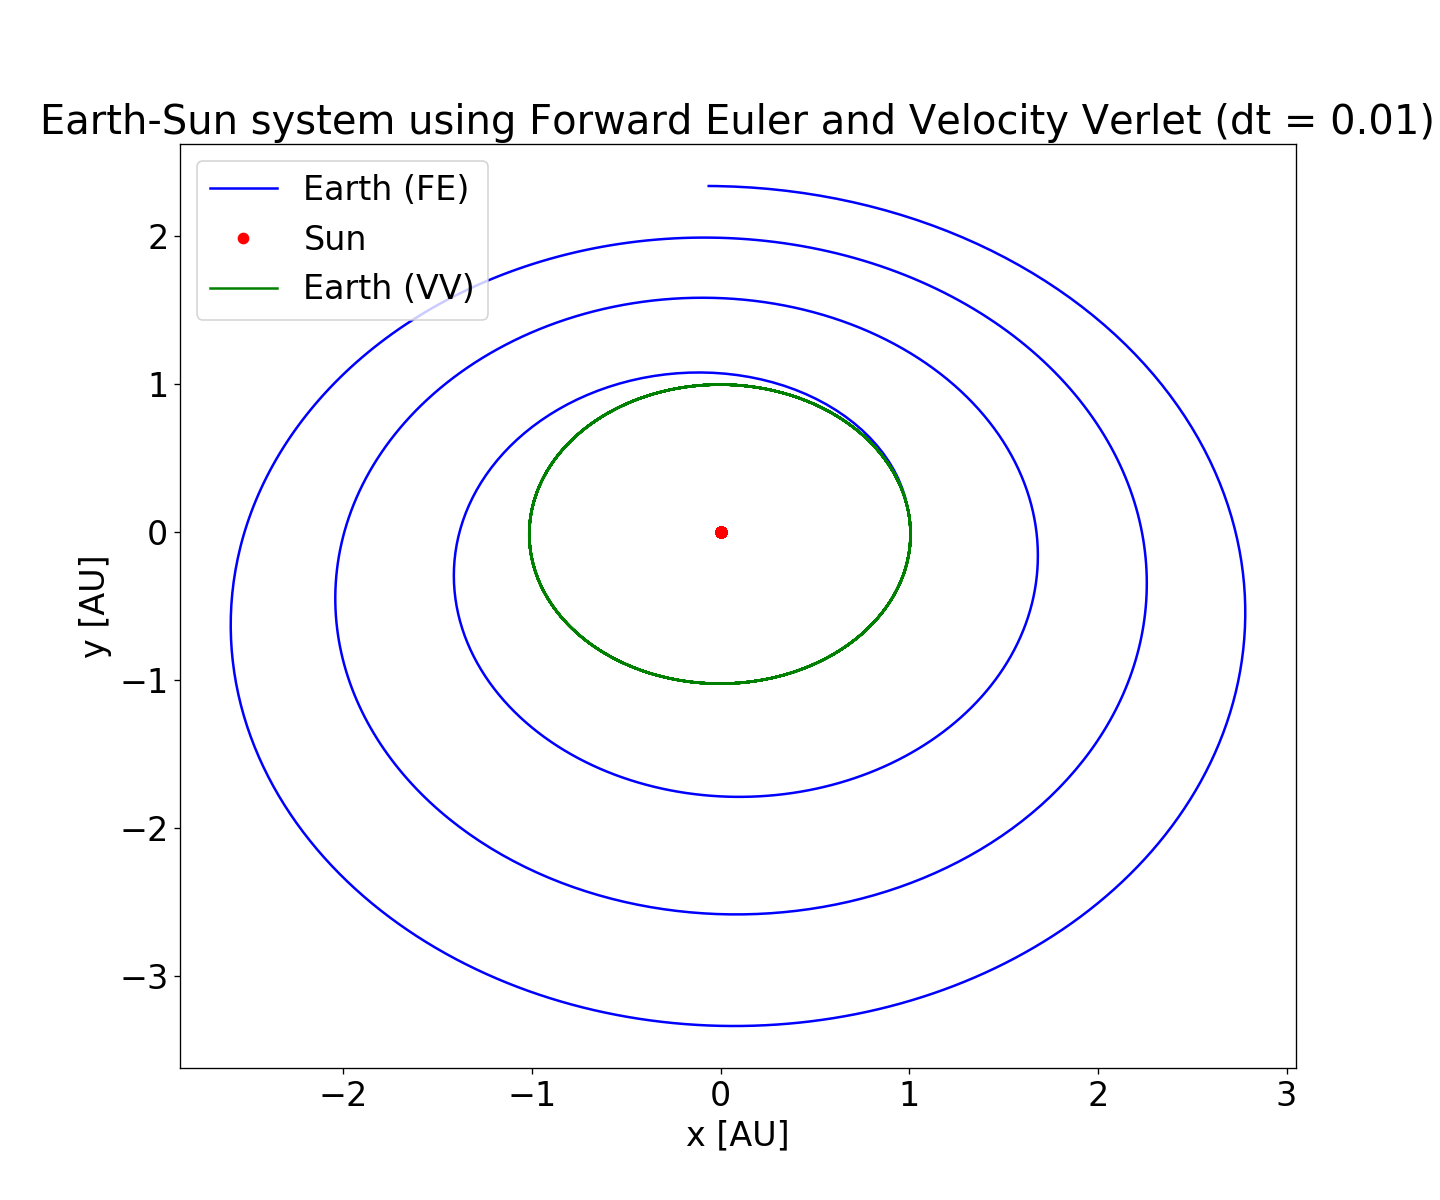
\includegraphics[width=\textwidth]{earth_sun_dt_001.png}
               
            \label{fig:comparison_dt0.01}
        \end{subfigure}
                \quad
        \begin{subfigure}[]{0.430\textwidth}  
            \centering 
            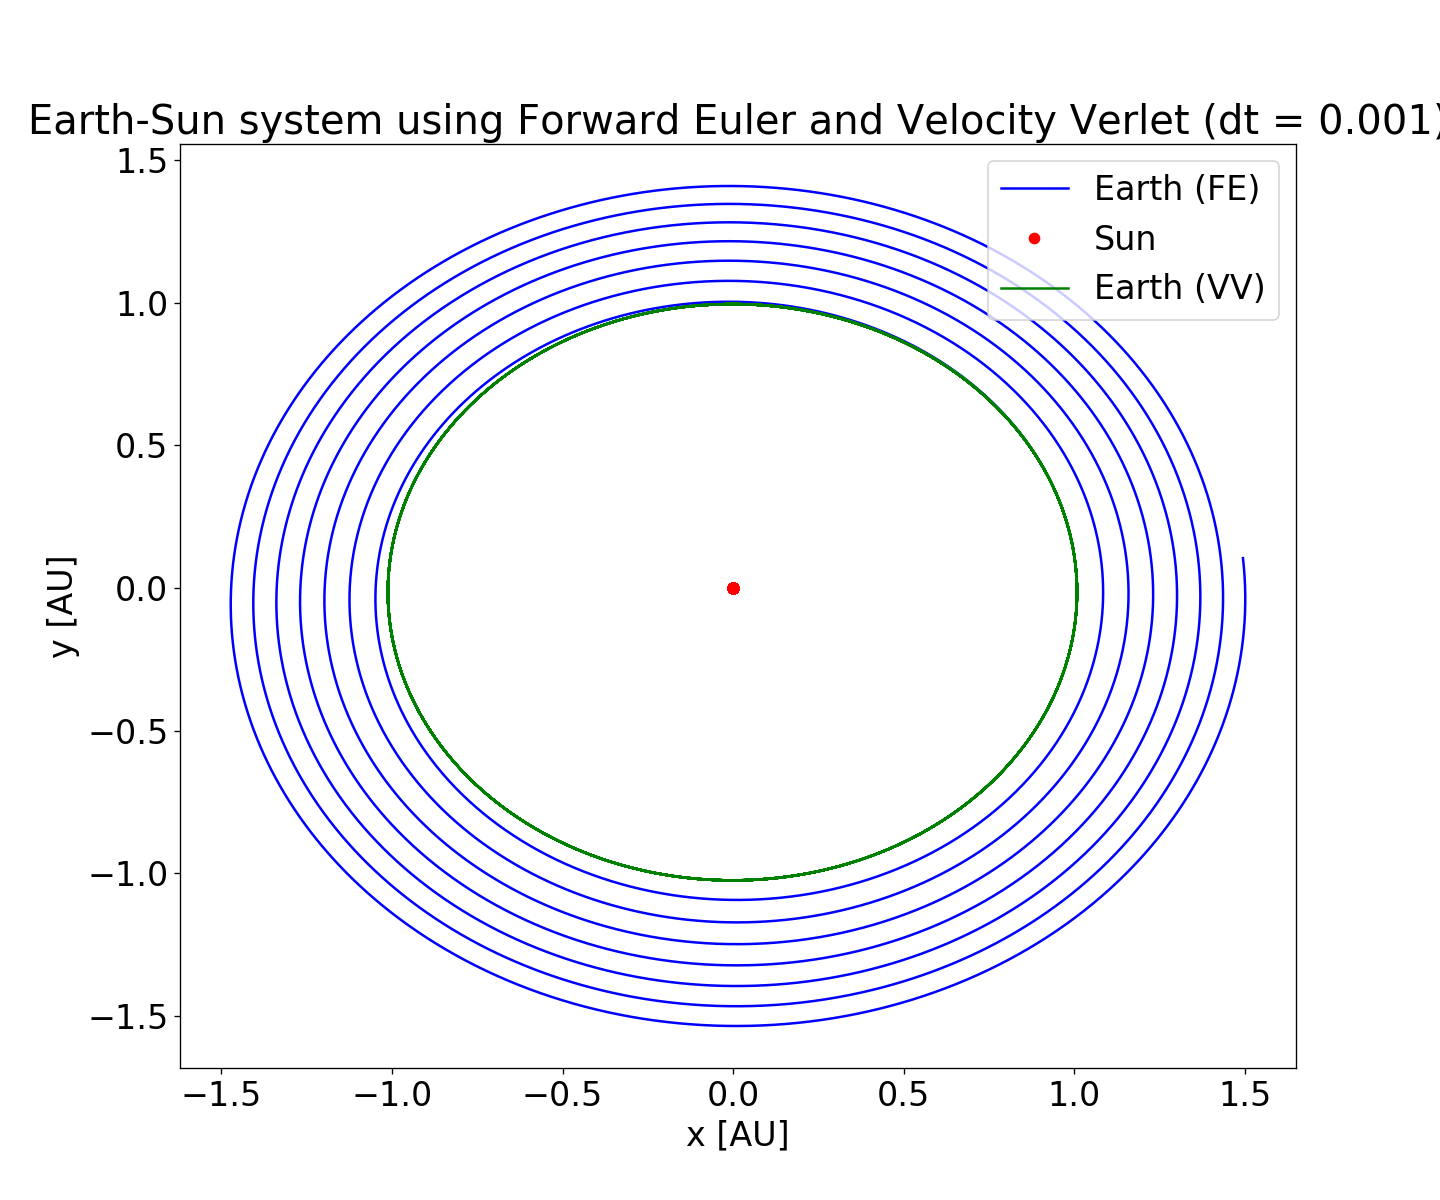
\includegraphics[width=\textwidth]{earth_sun_dt_0001.png}
                
            \label{fig:comparison_dt0.001}
        \end{subfigure}
        \vskip\baselineskip
        \begin{subfigure}[]{0.430\textwidth}   
            \centering 
            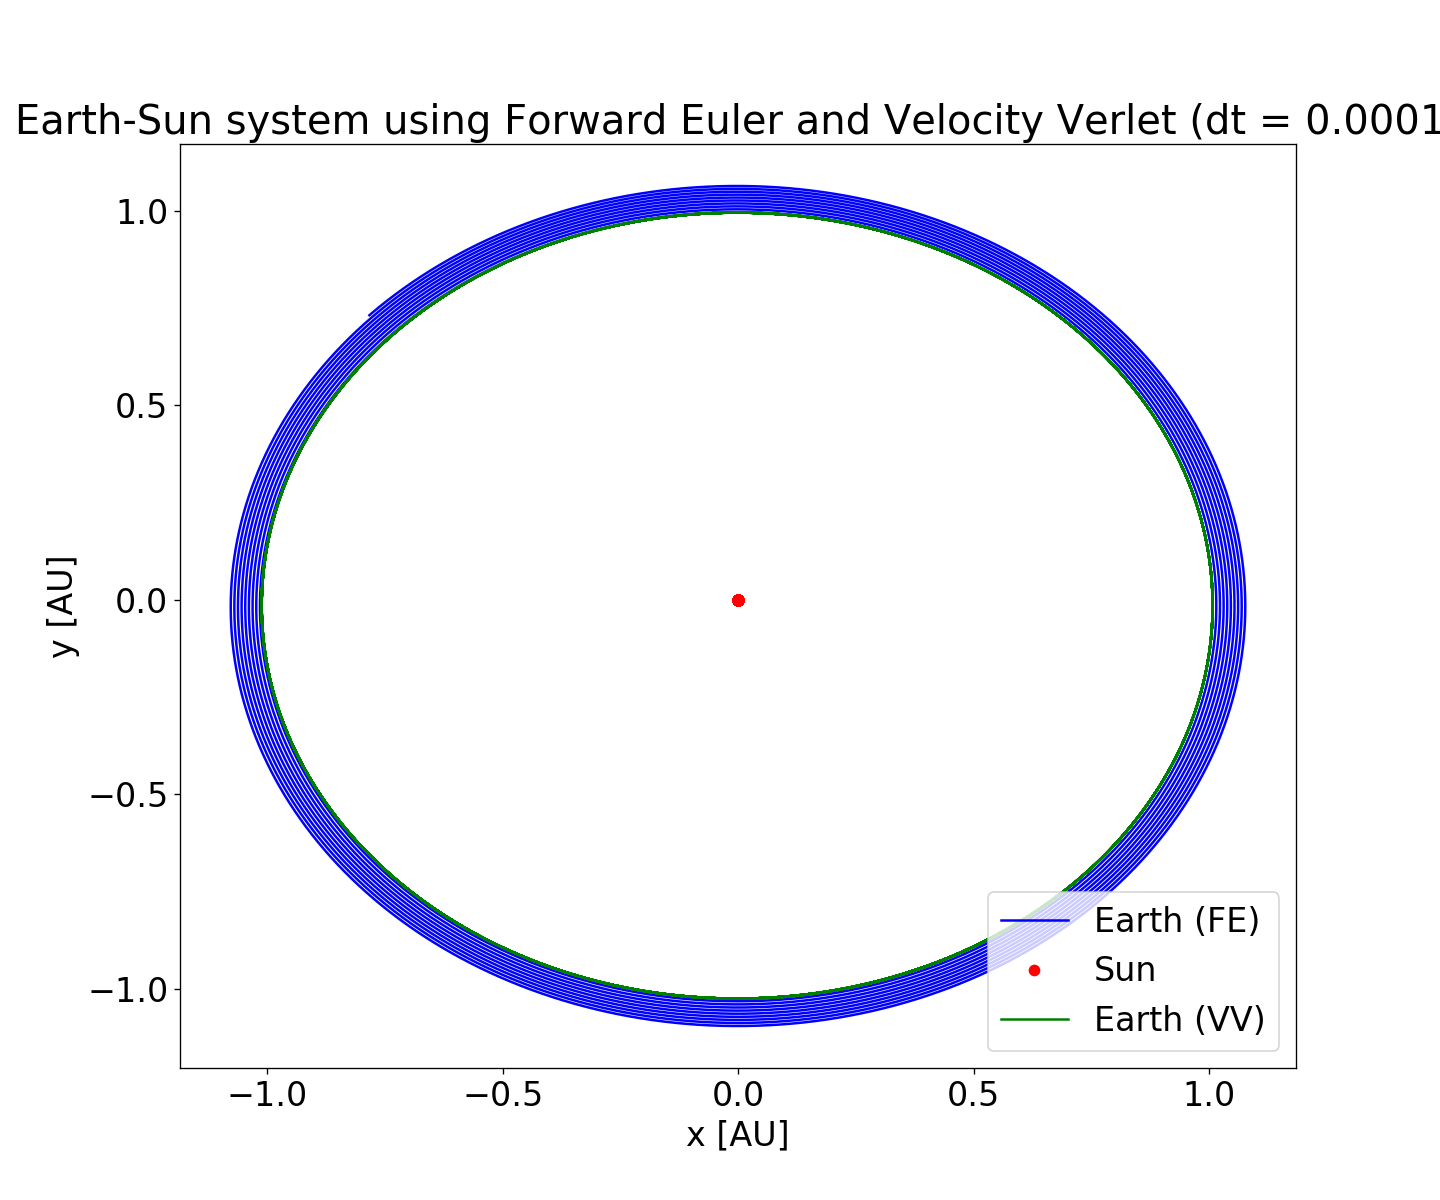
\includegraphics[width=\textwidth]{earth_sun_dt_00001.png}
                
            \label{fig:comparison_dt0.0001}
        \end{subfigure}
        \quad
        \begin{subfigure}[]{0.430\textwidth}   
            \centering 
            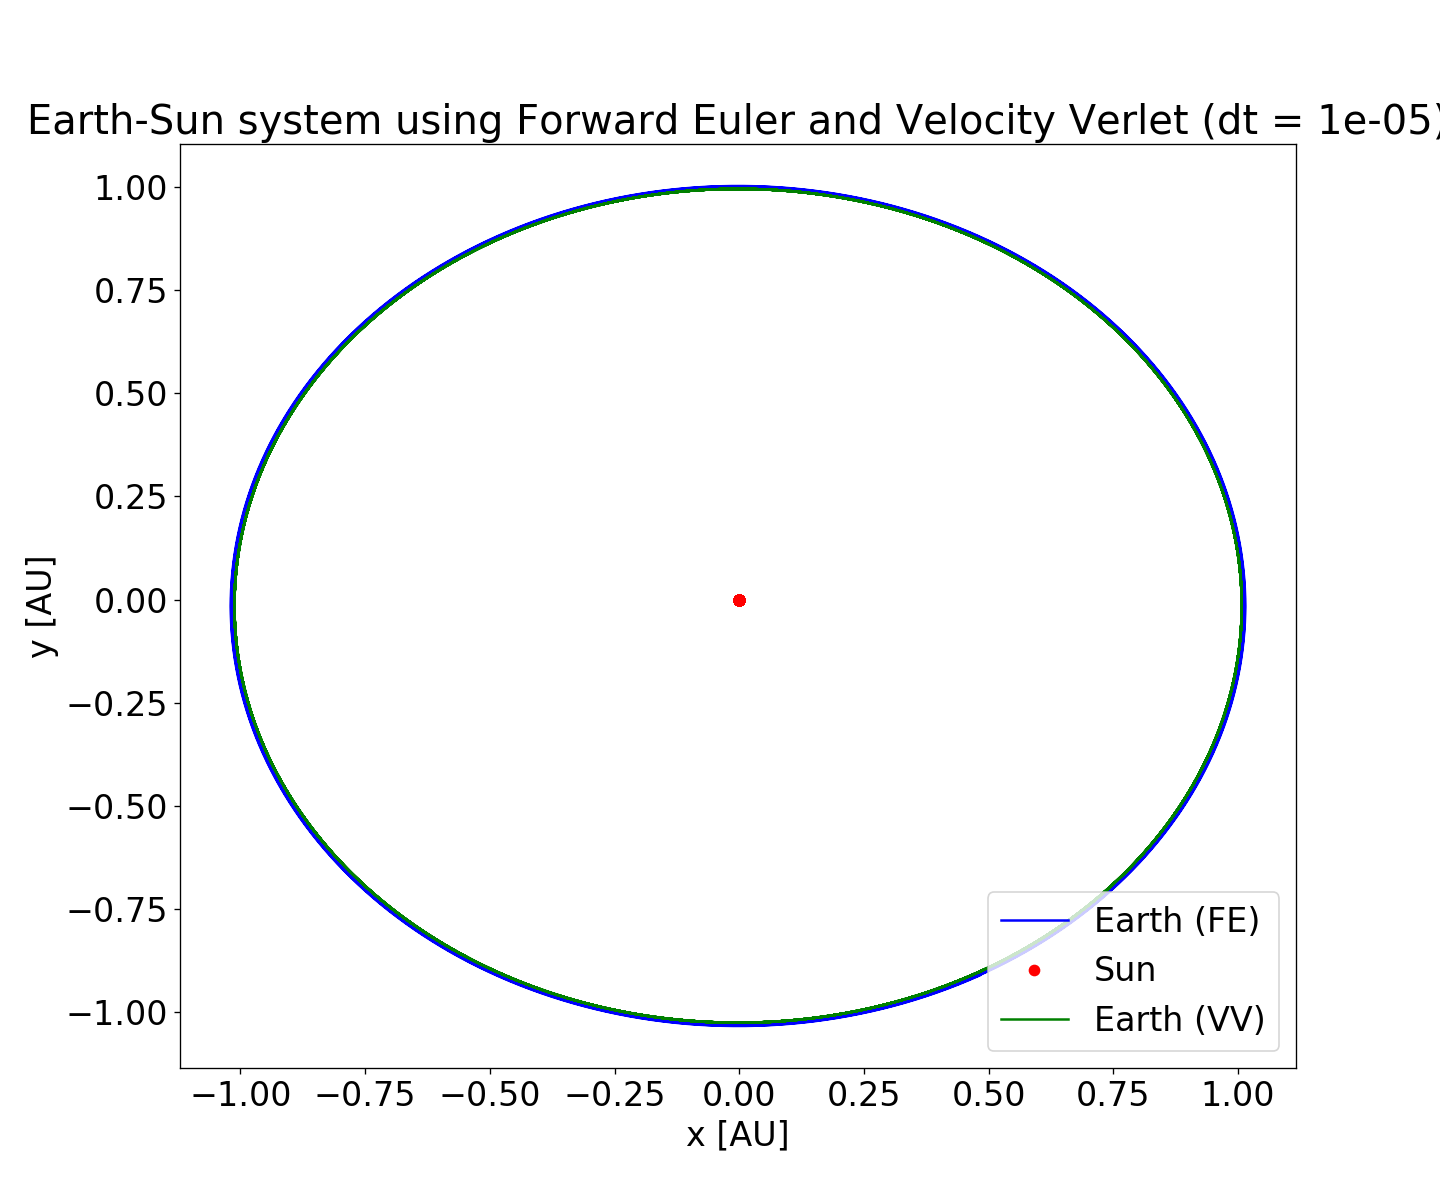
\includegraphics[width=\textwidth]{earth_sun_dt_1e-05.png}
              
            \label{fig:comparison_dt0.00001}
        \end{subfigure}
        \caption[]
        {\small The figure shows calculations of the Earth's orbit around the sun using the Euler Forward and Velocity Verlet algorithms for different time steps. As seen in the figure, Earth's orbit is stable using Verlet for all time steps. The orbit calculated by Forward Euler is not at all stable at large time steps, but improves towards $dt$ = 1e-05. } 
        \label{fig:2bodycomparison}
    \end{figure}
    
    
    
\subsubsection{Conservation of energy and angular momentum}
In figure (\ref{fig:energy_cons}), the different energies for the system is plotted for both algorithms over a time period of 10 years. To the left, one can see that the Velocity Verlet algorithm correctly conserves all energies after 10 years. The Forward Euler, however, does not conserve the energies. This is confirmed on the plot to the right where the relative total energy is plotted. It was also expected as the Earth was spiralling out of its orbit during the calculations.

In figure (\ref{fig:cons_ang}), the total angular momentum is plotted for both algorithms over a time period of 10 years. The angular momentum for the Velocity Verlet algorithm shows a horizontal line, while it shows an increasing angular momentum for the Forward Euler algorithm. It is thus only conserved for the Velocity Verlet algorithm.


\begin{figure}[]

        \centering
        \begin{subfigure}[]{0.485\textwidth}
            \centering
            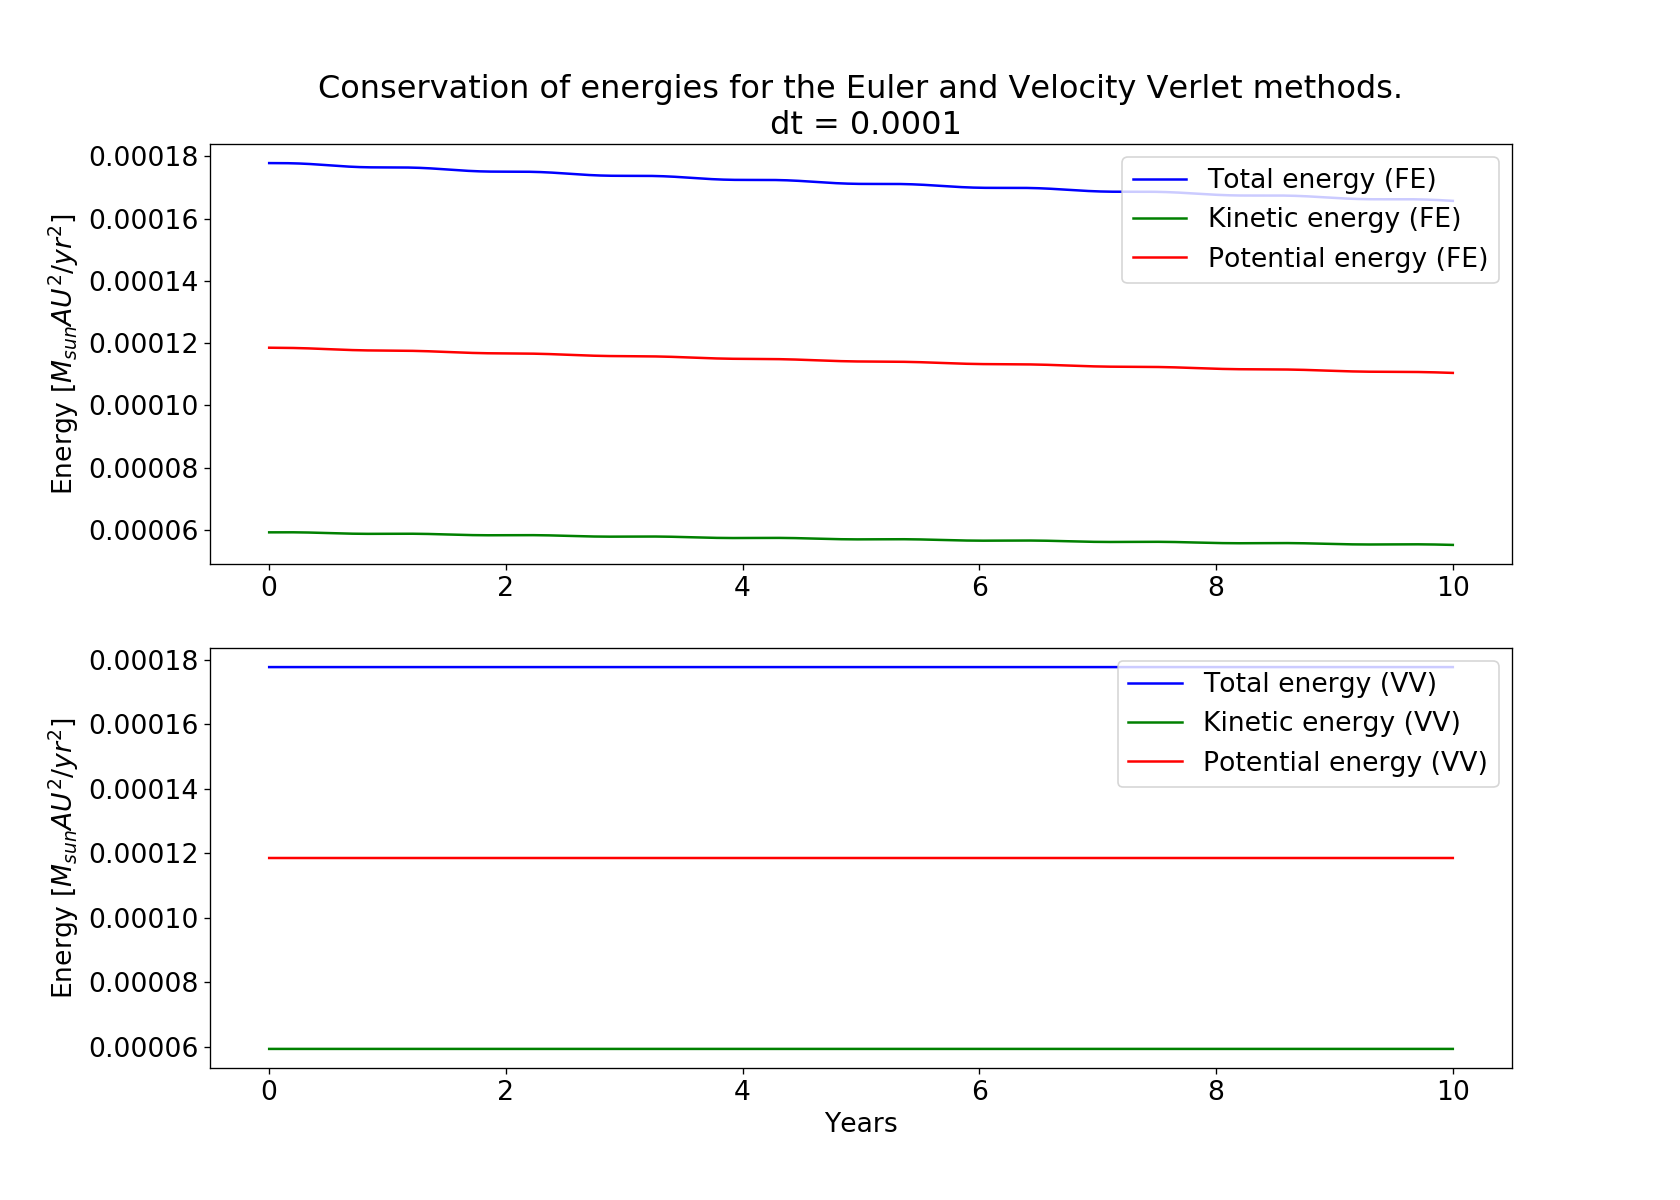
\includegraphics[width=\textwidth]{cons_E_dt_00001_f.png}
               
            \label{fig:E}
        \end{subfigure}
                \quad
        \begin{subfigure}[]{0.485\textwidth}  
            \centering 
            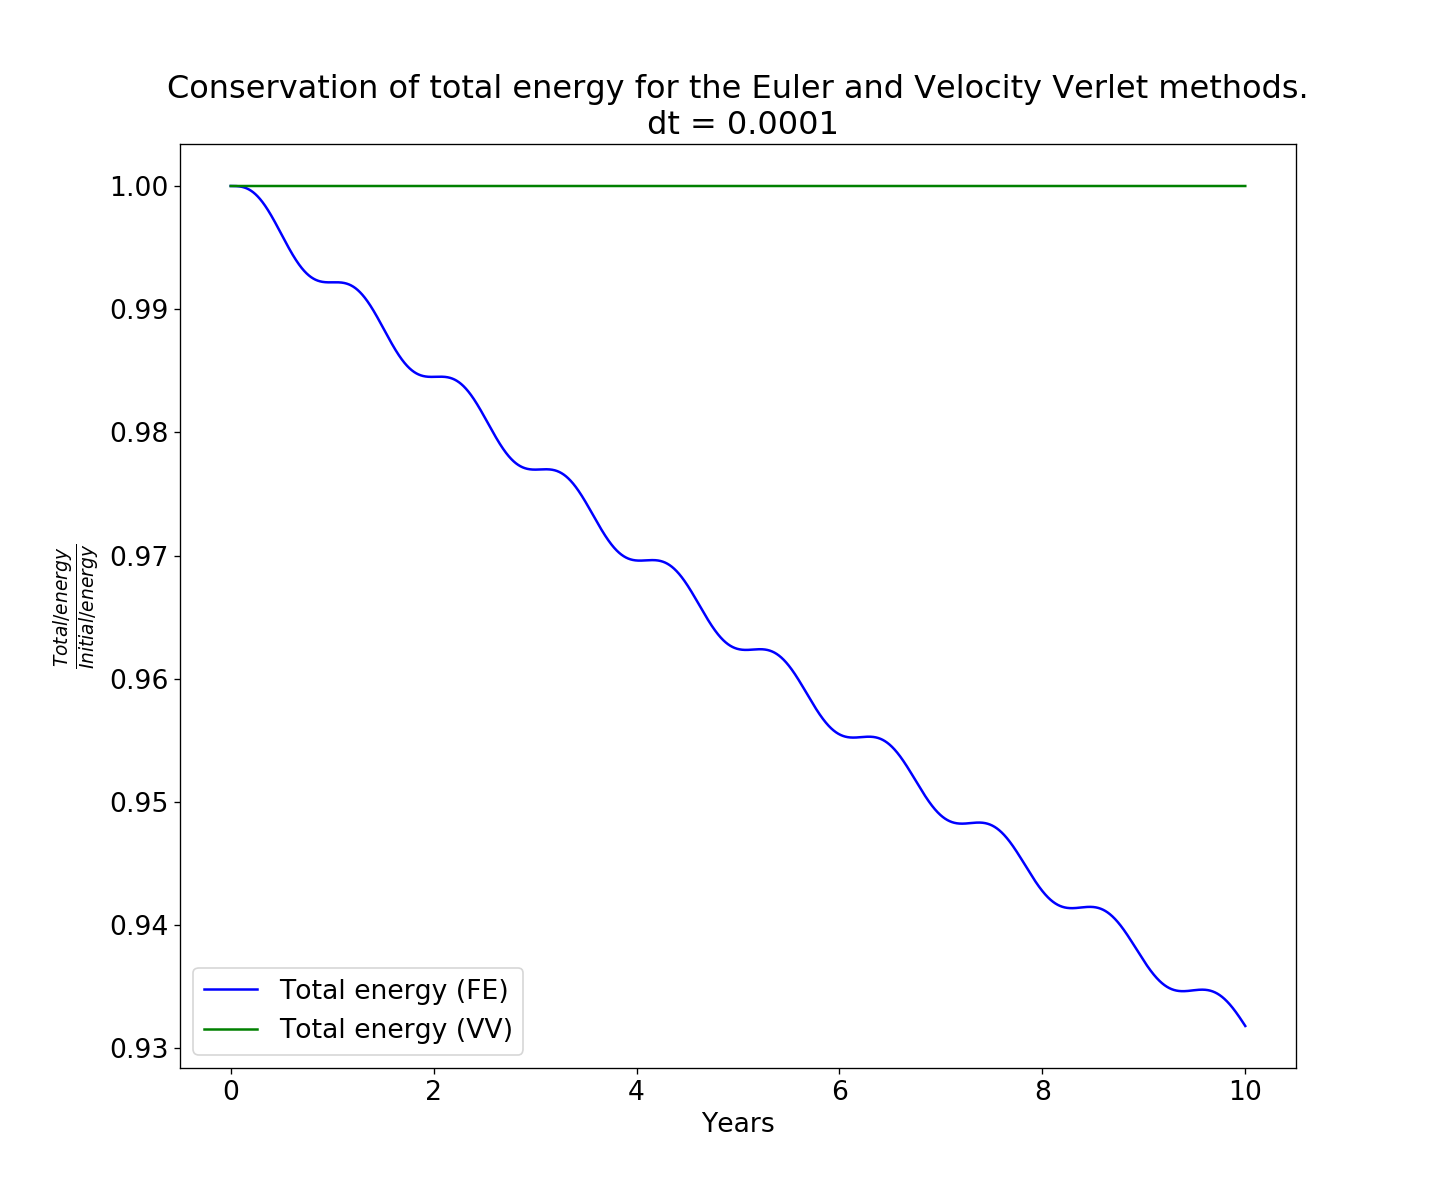
\includegraphics[width=\textwidth]{cons_E_rel_dt_00001_f2_smallerfont.png}
                
            \label{fig:E_rel}
        \end{subfigure}
        \vskip\baselineskip
        \caption[]
        {\small The figure to the left shows the conservation of total energy, kinetic energy and potential energy for both the Forward Euler algorithm (top) and the Velocity Verlet algorithm (bottom). On the right, the  relative total energy for both algorithms are shown. Both figures indicates that the Forward Euler does not conserve energy, while the Velocity Verlet does. This one reason why the latter method is used throughout this project.} 
        \label{fig:energy_cons}
    \end{figure}

\begin{figure}[]
\centering
\centering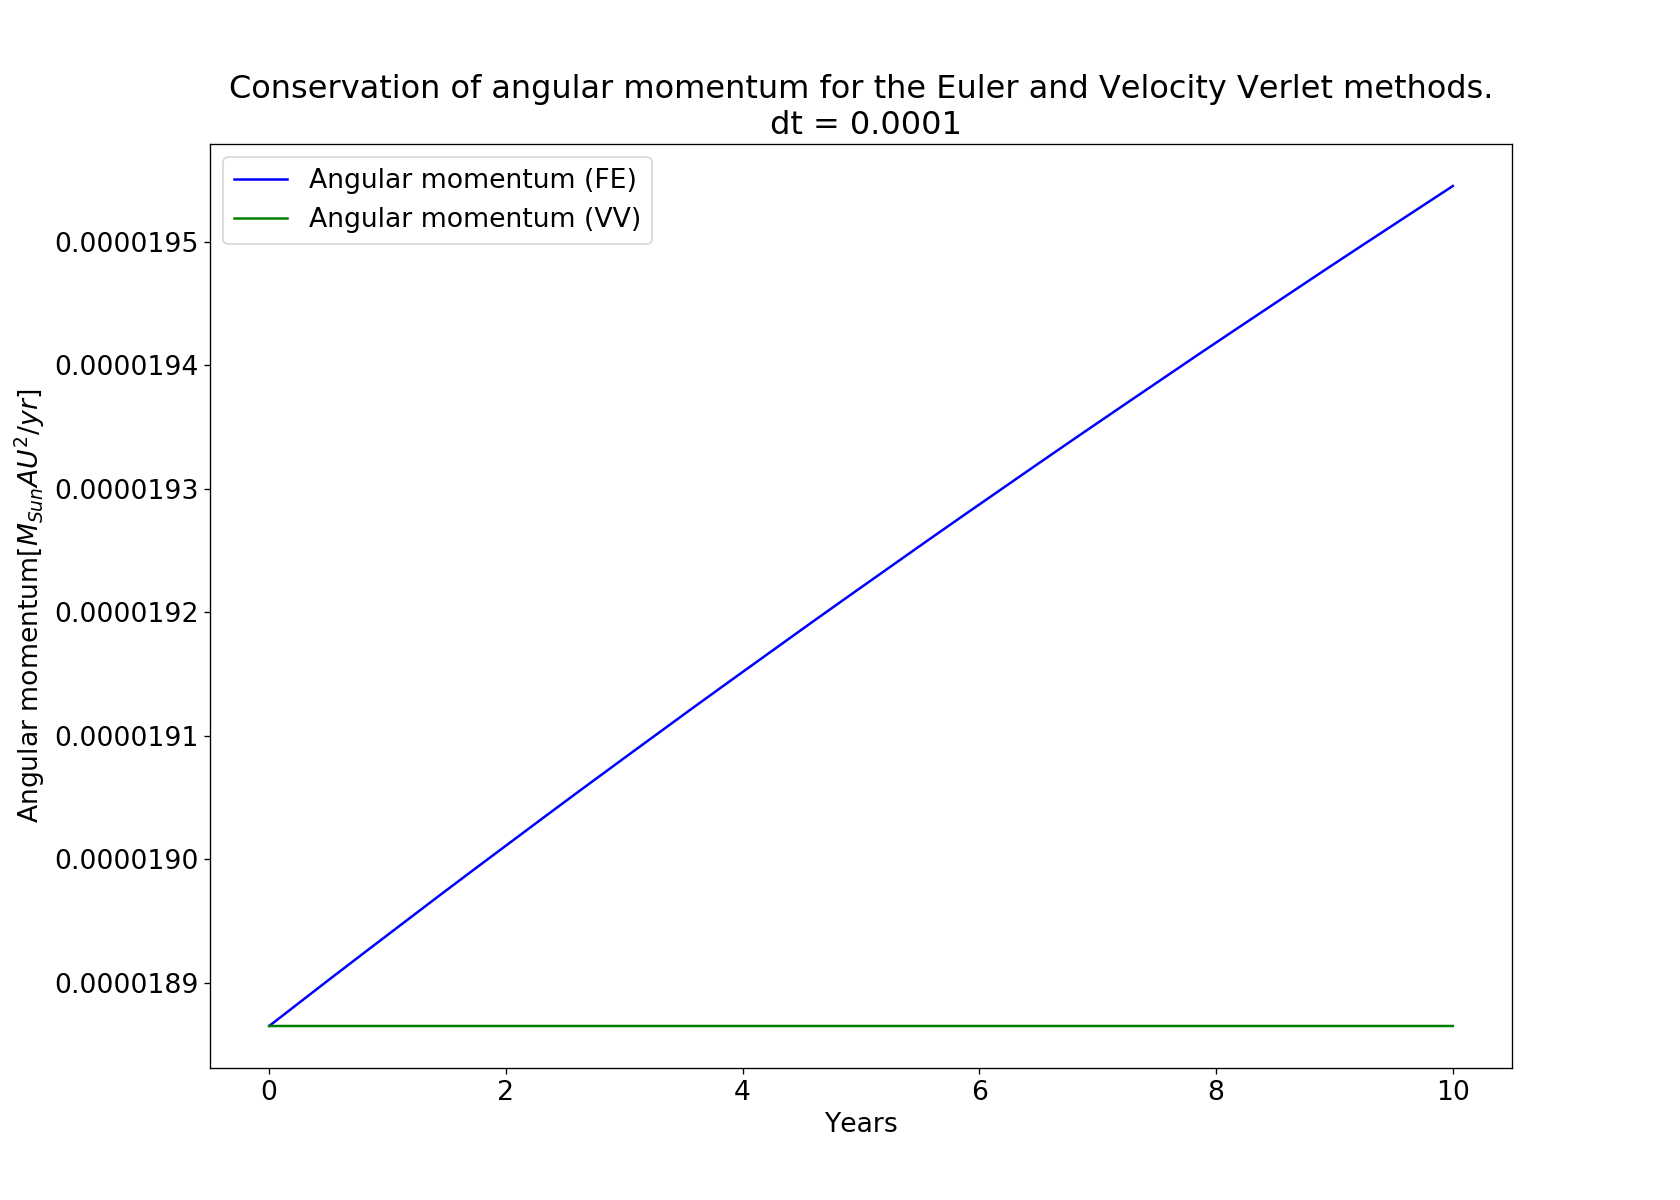
\includegraphics[scale=0.3]{cons_Ang_dt_00001_f.png}
\caption{The total angular momentum is here plotted for both algorithms. The angular momentum is conserved for the Velocity Verlet calculation, but it is not conserved for the Forward Euler calculation. \label{fig:cons_ang}}
\end{figure}

\subsubsection{Escape velocity}
With the sun fixed Sun at origin, the theoretical escape velocity was earlier calculated to be $v \approx$ 8.8857 AU/yr. To find the velocity numerically, several velocity values were tested to see if the Earth escaped from its orbit. The trials can be seen in figure (\ref{fig:escape}). Setting $k$ to 1.41 in the formula $v = k2\pi$ AU/yr seemed to make the planet escape its orbit. This equals a velocity of 8.8859 AU/yr, which is indeed close to the theoretical value. Velocities below the escape velocity induce elliptical orbits. 

\begin{figure}[]
\centering
\centering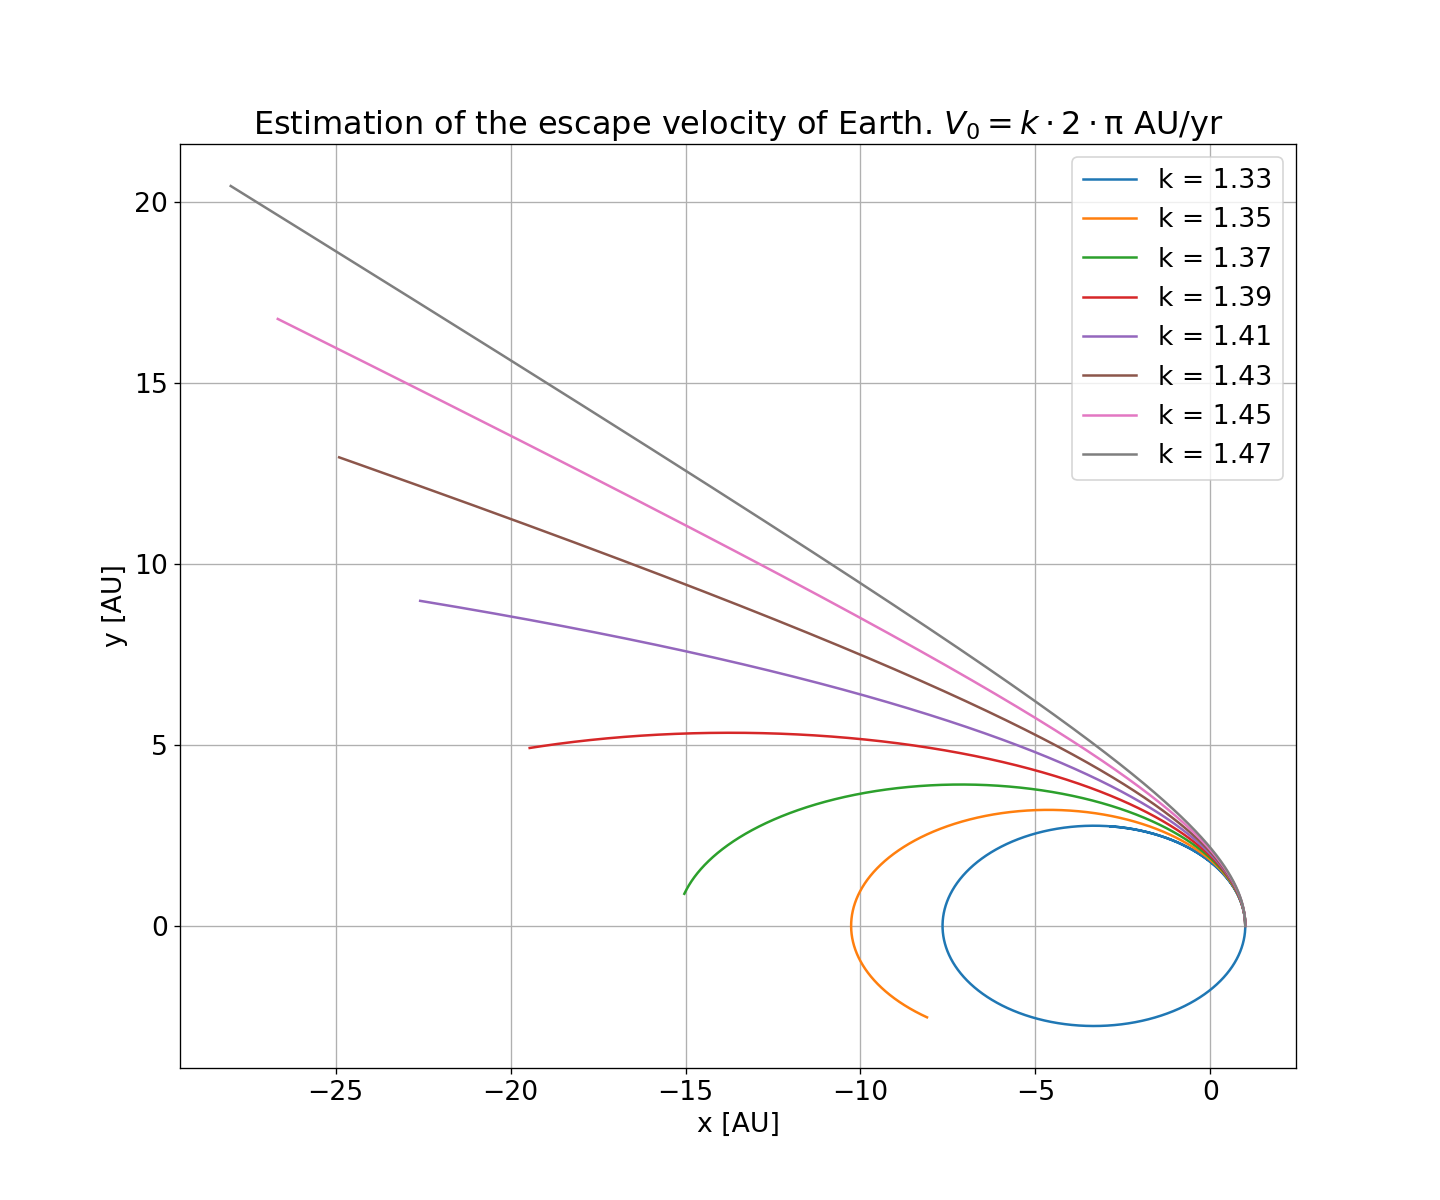
\includegraphics[scale=0.4]{escape_velocity_dt_00001.png}
\caption{The figure shows the orbit of the earth with different initial velocities determined by a constant $k$. The value 1.41 (8.8859 AU/yr) seems to make earth escape. This value is close to the theoretical value of 8.8857 AU/yr. \label{fig:escape}}
\end{figure}

In addition to experimenting with increasing initial velocities, a calculation with a weaker gravitational force were done on the Earth-Sun System. With a gravitational force going as $1/r^3$ instead of $1/r^2$, the earth started spiralling out. This can be seen in figure (\ref{fig:weaker}).

\begin{figure}[]
\centering
\centering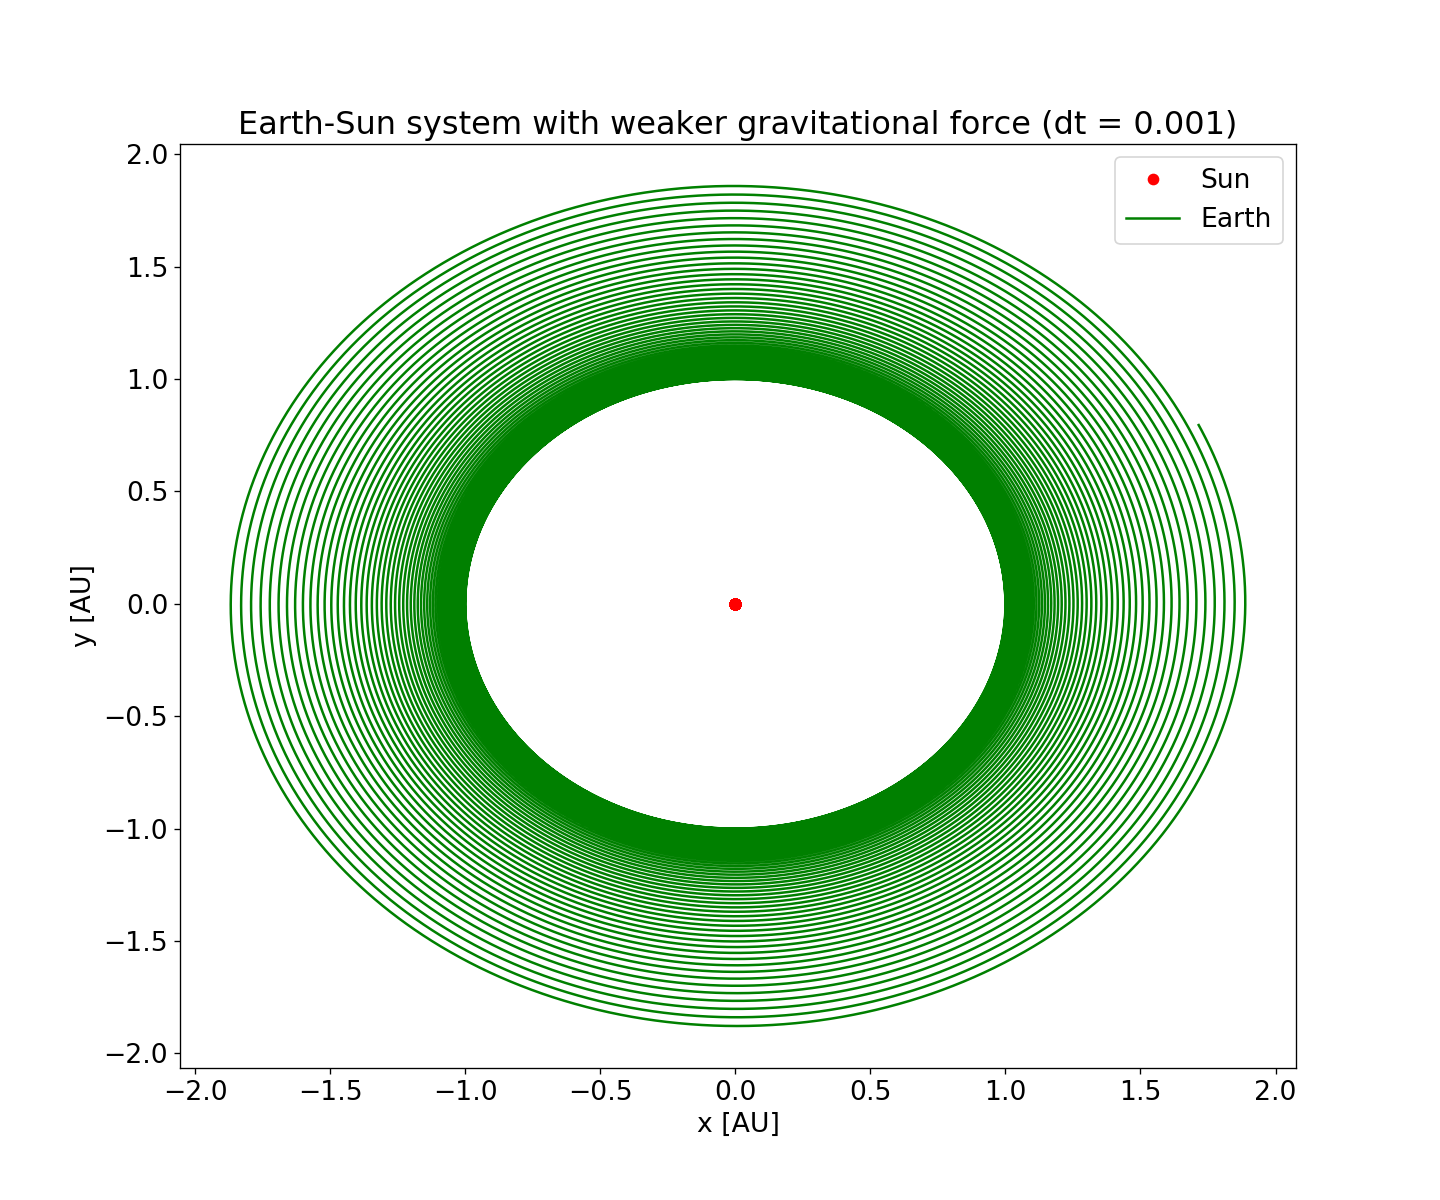
\includegraphics[scale=0.4]{weaker_grav_dt_0001.png}
\caption{Earth-Sun system simulated for 100 years with weaker gravitational force. The force is now not strong enough to keep Earth in orbit. \label{fig:weaker}}
\end{figure}

\subsection{Earth-Sun-Jupiter system}
Adding Jupiter to the system turns the problem into a three-body problem. Because Jupiter is the largest planet in the solar system, it may effect the orbits of other planets. The Velocity Verlet algorithm were in this part used to find Jupiter's impact on Earth's orbit with a time step of 0.0001. This was done both with a stationary Sun and with a moving Sun. Jupiter's mass was increased from its realistic mass to a mass 10 and 1000 times its original mass. 

The Sun is around 1 AU away from the Earth, while Jupiter is around 5.20 AU away from the sun. Because the gravitational force goes as $1/r^2$, the change in the Earth's orbit is mainly from the change in the Sun's position because of the gravitational force of Jupiter, and not from Jupiter directly. 

In figure (\ref{fig:jupiter_only}), the three-body system is shown with and without a stationary Sun. A slight shift in the positions of the bodies can be seen from the addition of Jupiter when the Sun is free to move (left). When the Sun is stationary (right), however, no shift in positions can be seen. This is because of, as mentioned, Jupiter's indirect influence on Earth's orbit.

Figure (\ref{fig:jupiter_fixed}) shows Earth's orbits for different Jupiter masses with the sun fixed. Earth's orbit is still stable when increasing Jupiter's mass tenfold, and the change in orbit is difficult to spot on this scale. Increasing Jupiter's mass thousandfold makes the orbit of the Earth unstable. 

Figure (\ref{fig:jupiter}) shows the same, but with a moving Sun. Now, it is easier to see Jupiter's influence on Earth's orbit. When Jupiter's mass is set to 1000 times its original mass, the Earth is sent out of orbit. The Sun and Jupiter now has approximately the same mass, and will start to orbit around a new center of mass. 

\begin{figure}[]

        \centering
        \begin{subfigure}[ht]{0.485\textwidth}
            \centering
            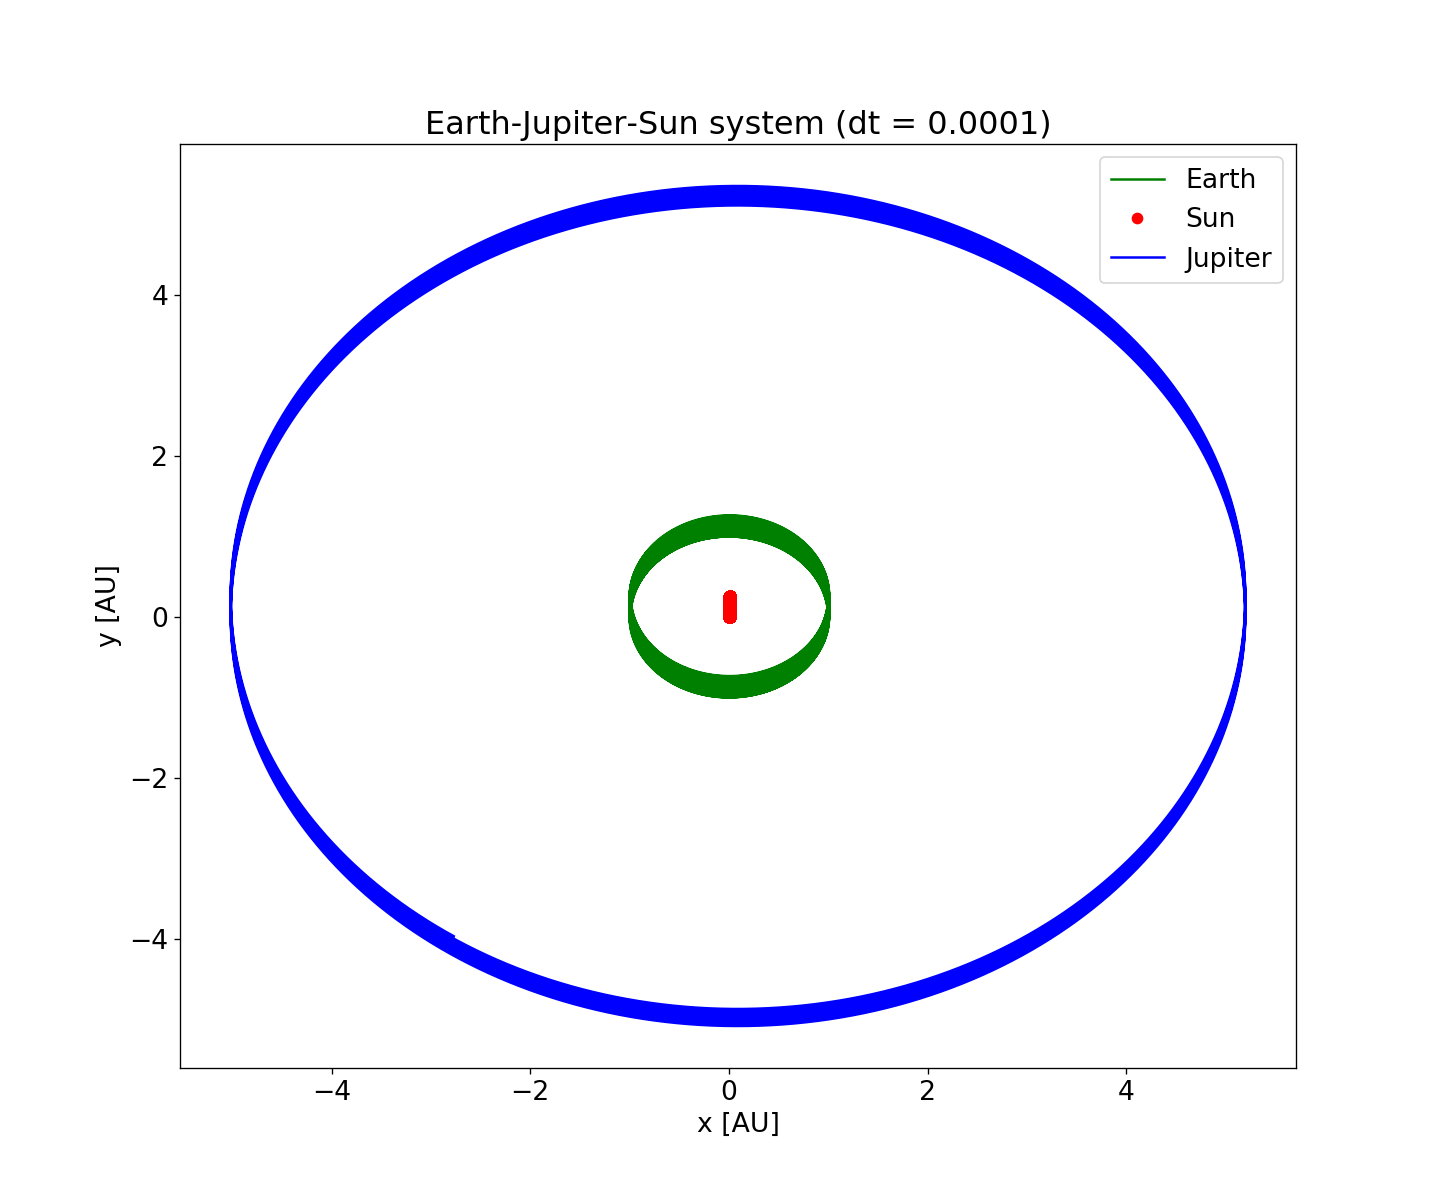
\includegraphics[width=\textwidth]{earth_jupiter_notfixed_dt_00001.png}
               
            \label{fig:jupnot}
        \end{subfigure}
                \quad
        \begin{subfigure}[ht]{0.485\textwidth}  
            \centering 
            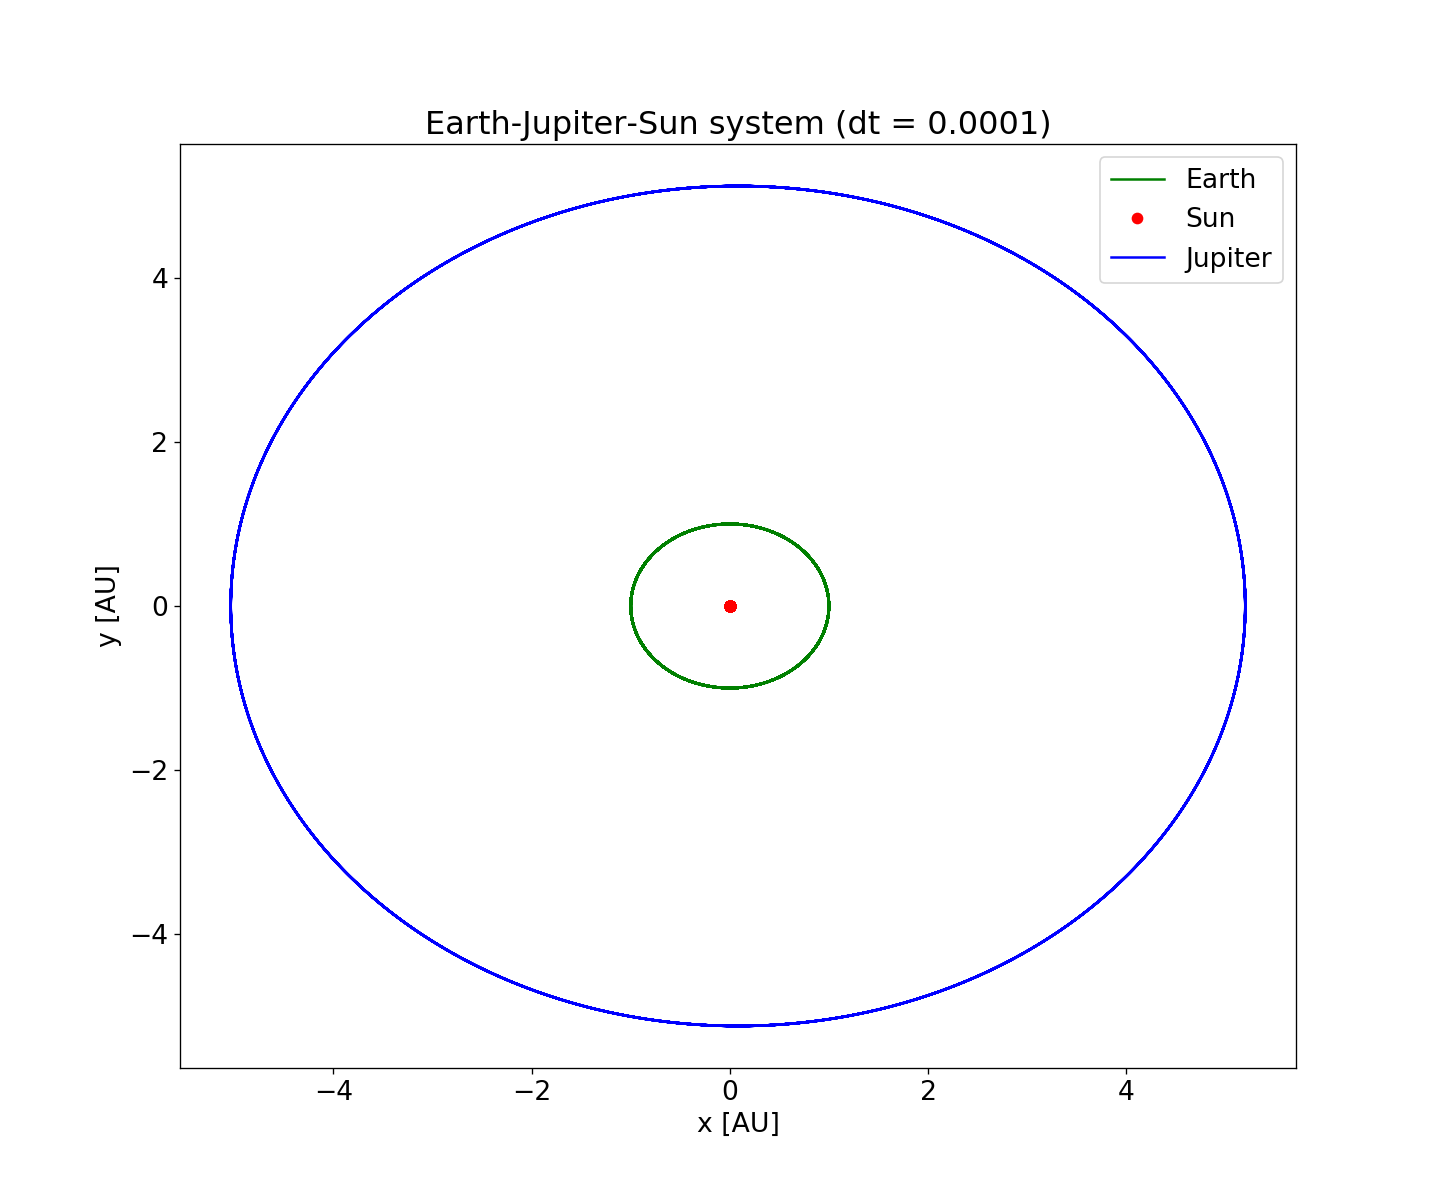
\includegraphics[width=\textwidth]{earth_jupiter_fixed_dt_00001.png}
                
            \label{fig:jupfix}
        \end{subfigure}
        \vskip\baselineskip
        \caption[]
        {\small Plots of the three-body problem around a moving Sun (left) and fixed Sun (right). The time step was set to 0.0001. One can here see the slight influence of the Orbits due to Jupiter's large mass when the Sun is free to move.} 
        \label{fig:jupiter_only}
    \end{figure}


\begin{figure}[]
\centering
\centering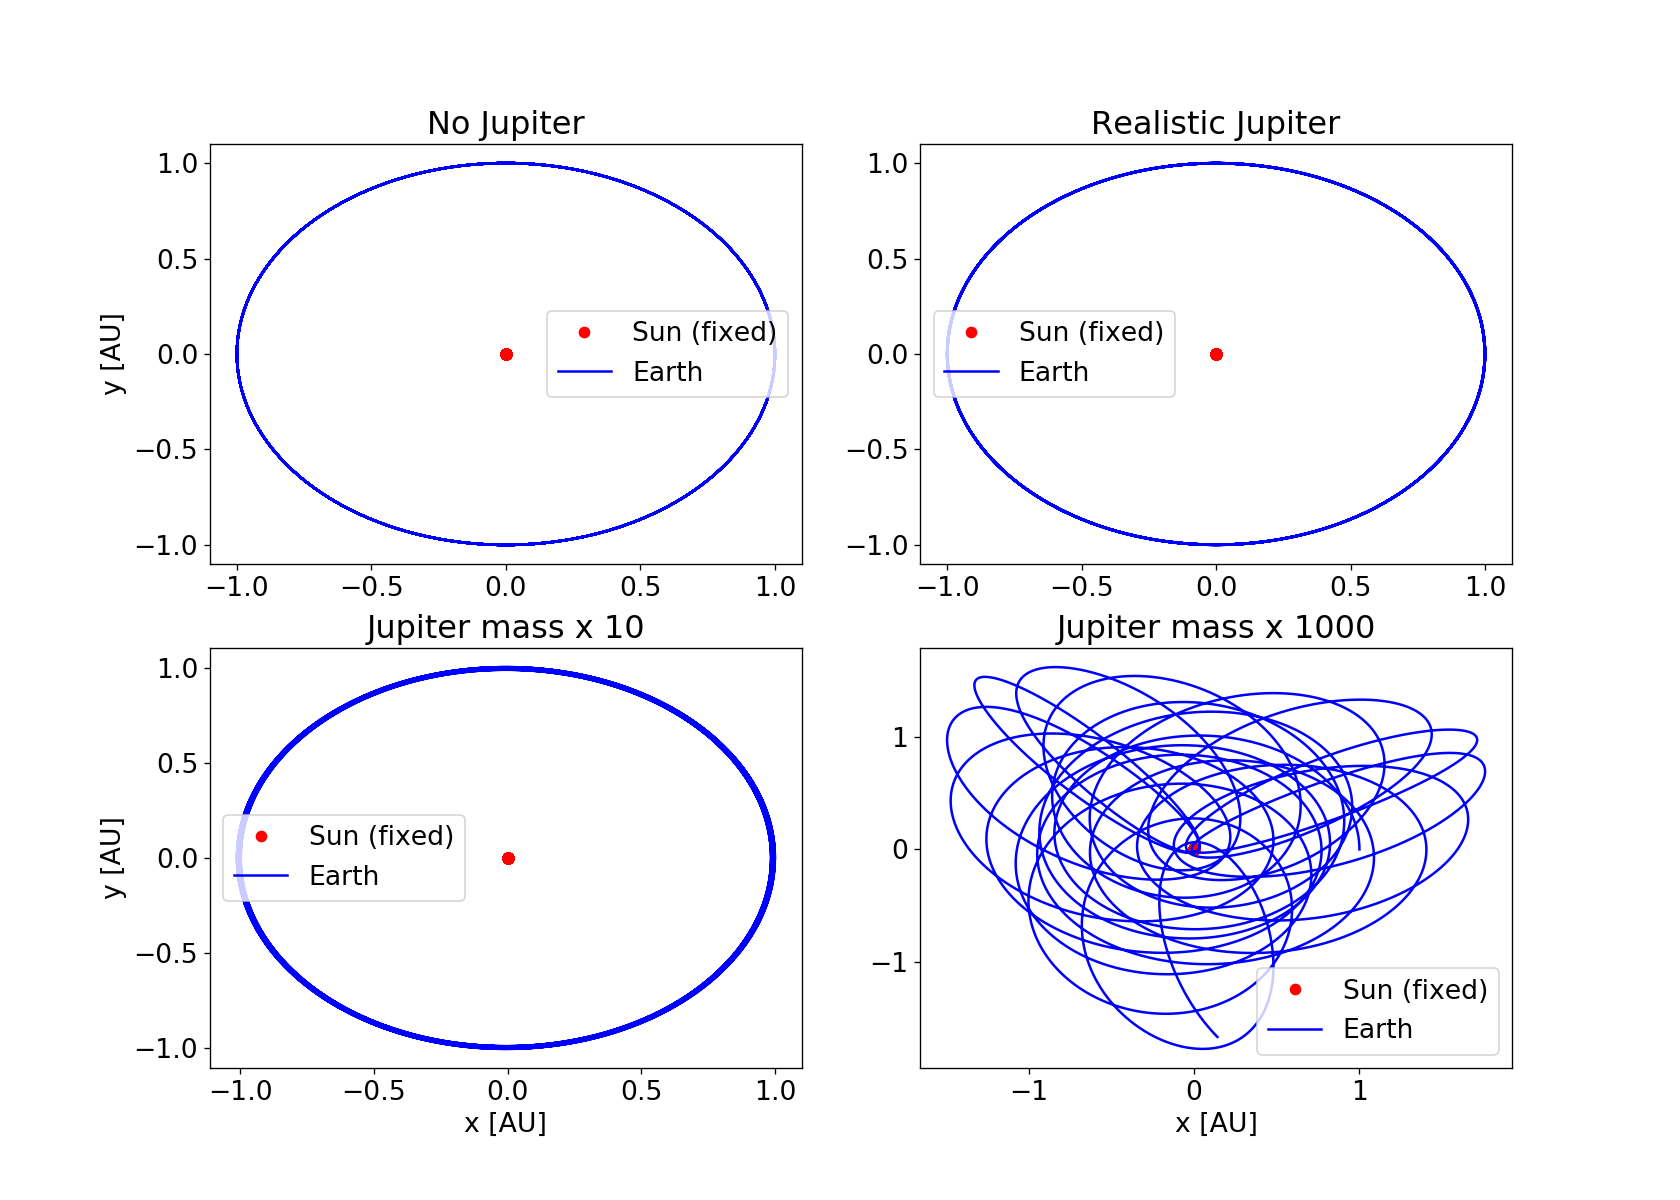
\includegraphics[scale=0.4]{jupiter_fixed_sun_dt_00001.png}
\caption{Plots of Earth's orbit around a stationary Sun with an increasing Jupiter mass. The time step was set to 0.0001. Earth's orbit it still stable at Jupiter's original mass times 10, but it becomes unstable when increased to 1000.  \label{fig:jupiter_fixed}}
\end{figure}

\begin{figure}[]
\centering
\centering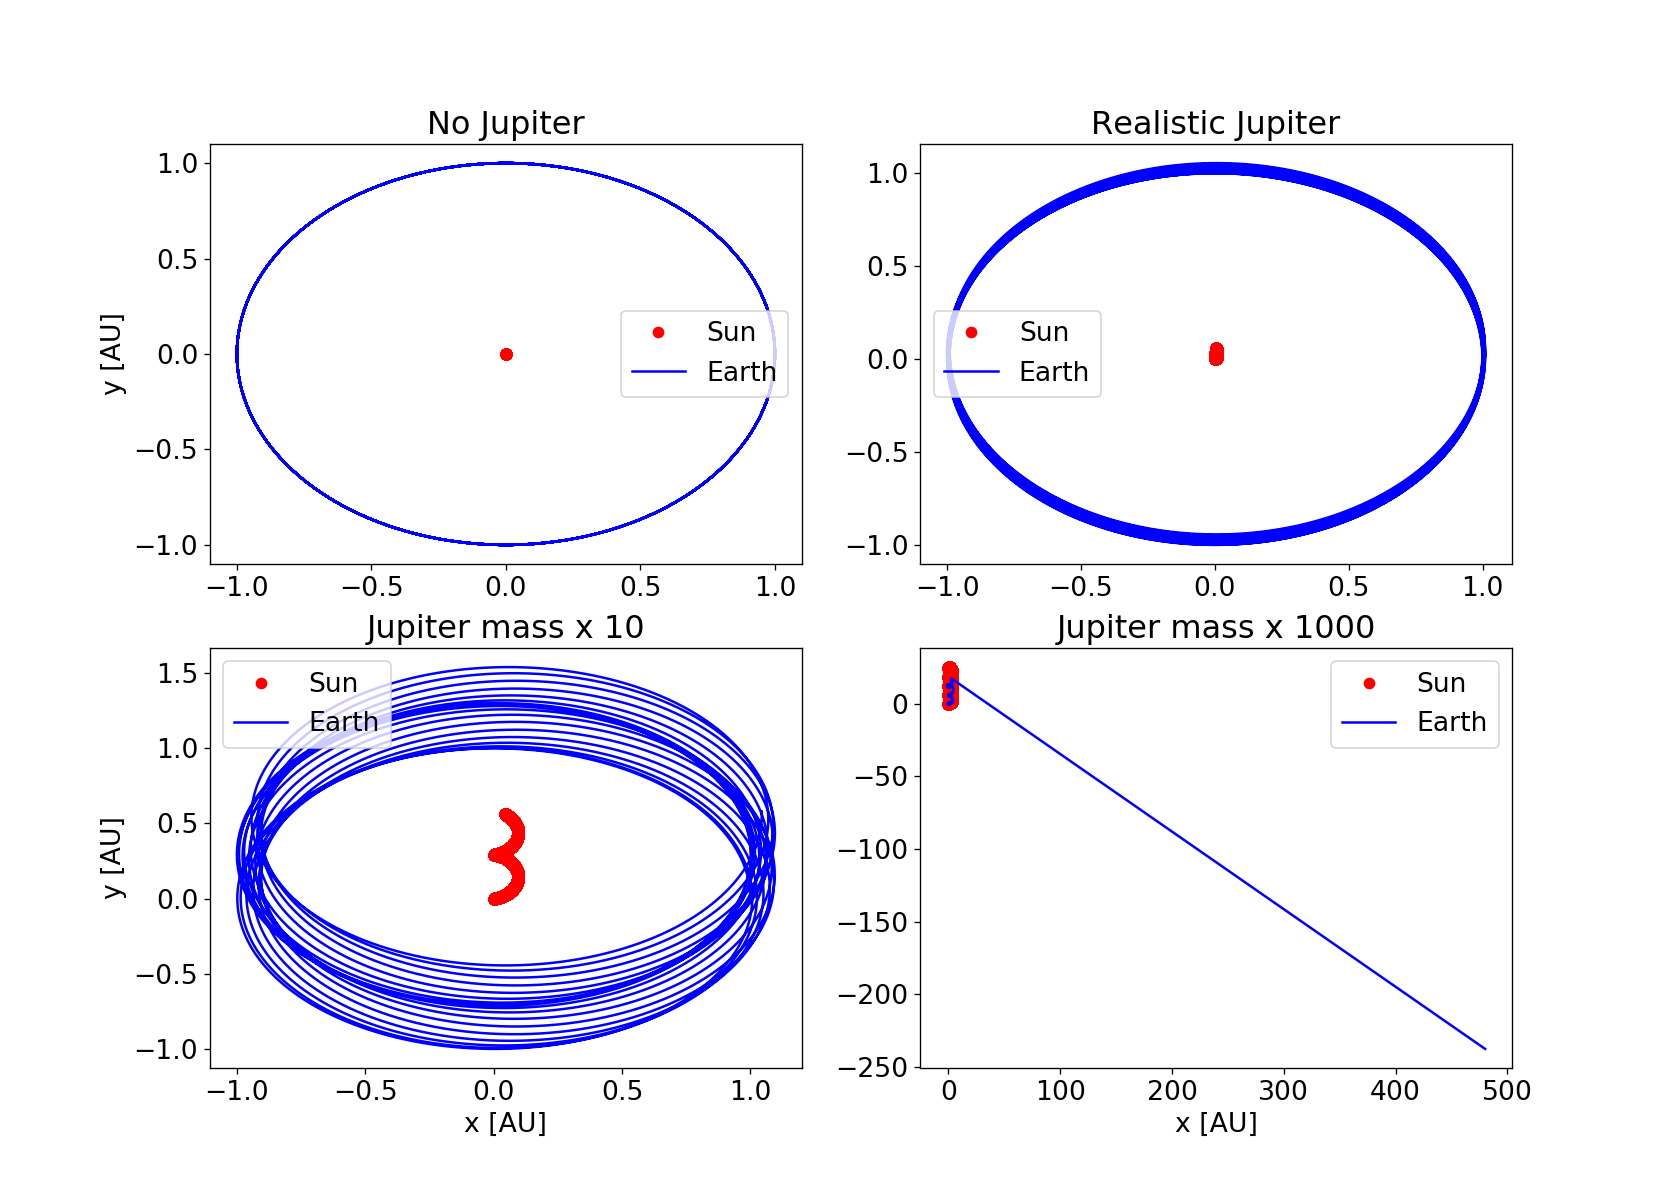
\includegraphics[scale=0.4]{jupiter_dt_00001.png}
\caption{Plots of Earth's orbit around a moving Sun with an increasing Jupiter mass. The time step was set to 0.0001. Earth's orbit is here disrubted when Jupiter's mass is increased tenfold. Increasing it shousandfold sends the Earth out of orbit.  \label{fig:jupiter}}
\end{figure}

\subsection{Full solar system}
Adding the rest of the planets, the problem turns into a 9-body problem. The orbits were calculated using the Velocity Verlet algorithm over 200 years with a time step of 0.001. This ensures that all planets do at least one full revolution around the Sun.The center-of-mass position was set to origin, and all the bodies were free to move. The Sun was given an initial velocity that made the total momentum of the system zero. The plot of the orbits can be seen in figure (\ref{fig:full_system}). Again, the Velocity Verlet algorithm produces stable orbits even with small time steps and many bodies. 

\begin{figure}[]
\centering
\centering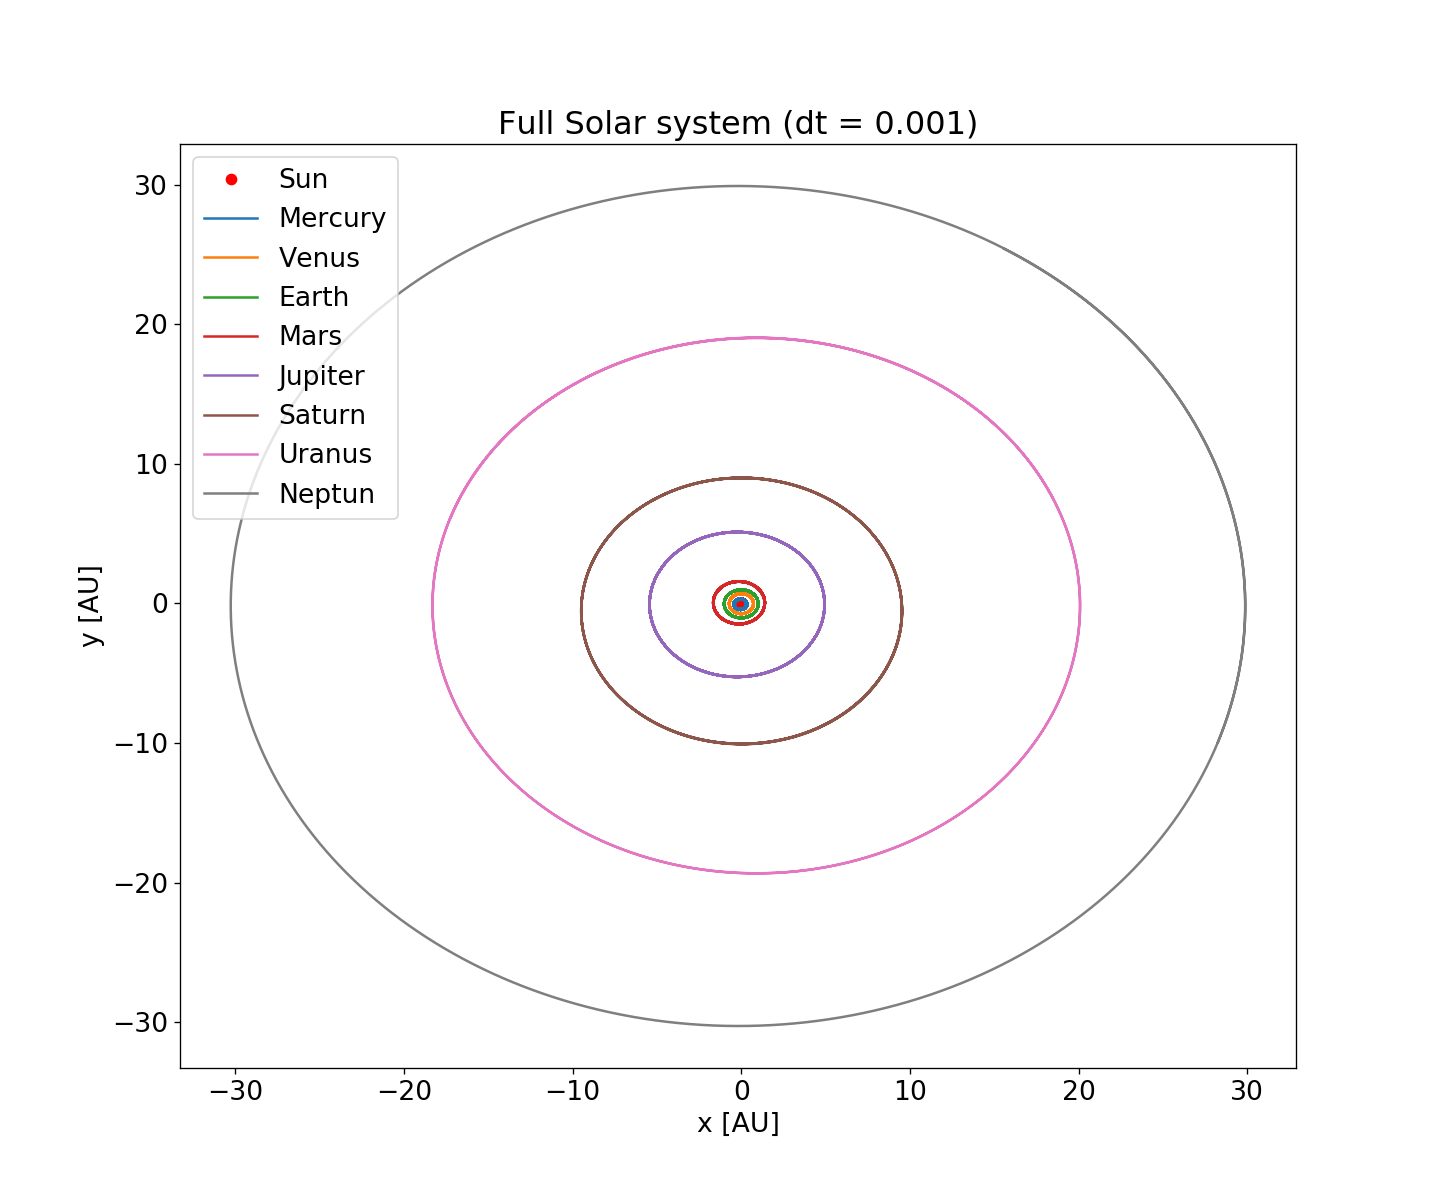
\includegraphics[scale=0.4]{full_system_dt_0001.png}
\caption{Plot of the full Solar Sytem over a period of 200 years with a time step of 0.001. All orbits seem stable despite the use of a small time step. Initial conditions from NASA were used. \label{fig:full_system}}
\end{figure}

\subsection{Perihelion precession of Mercury}
To observe the mentioned perihelion precession of Mercury, all other planets were removed from the simulation. First, the perihelion was calculated using the Newtonian force. The simulation was run over 100 years of orbiting while the perihelion's position was found by checking at each time step if the distance from the Sun was shorter than the previous and next distance. At each perihelion position, the angular position relative to the x-axis was calculated and converted to arcseconds. Mercury's initial position was set to its perihelion (0.3075 AU from the sun at a speed of 12.44 AU/yr). The same calculation were done with the force corrected for general relativity, and the angular positions in arcseconds for both simulations were plotted against time in Mercury years. The plot can be seen in figure (\ref{fig:mercury}). The time step used is not small enough to determine the perihelion with high precision, but the trend is still clearly visible.

The calculated angular velocity was found to be around 43 arcseconds per century, which fits with observations and predictions from general relativity. This is one way of confirming Einstein's theory of general relativity.

\begin{figure}[]
\centering
\centering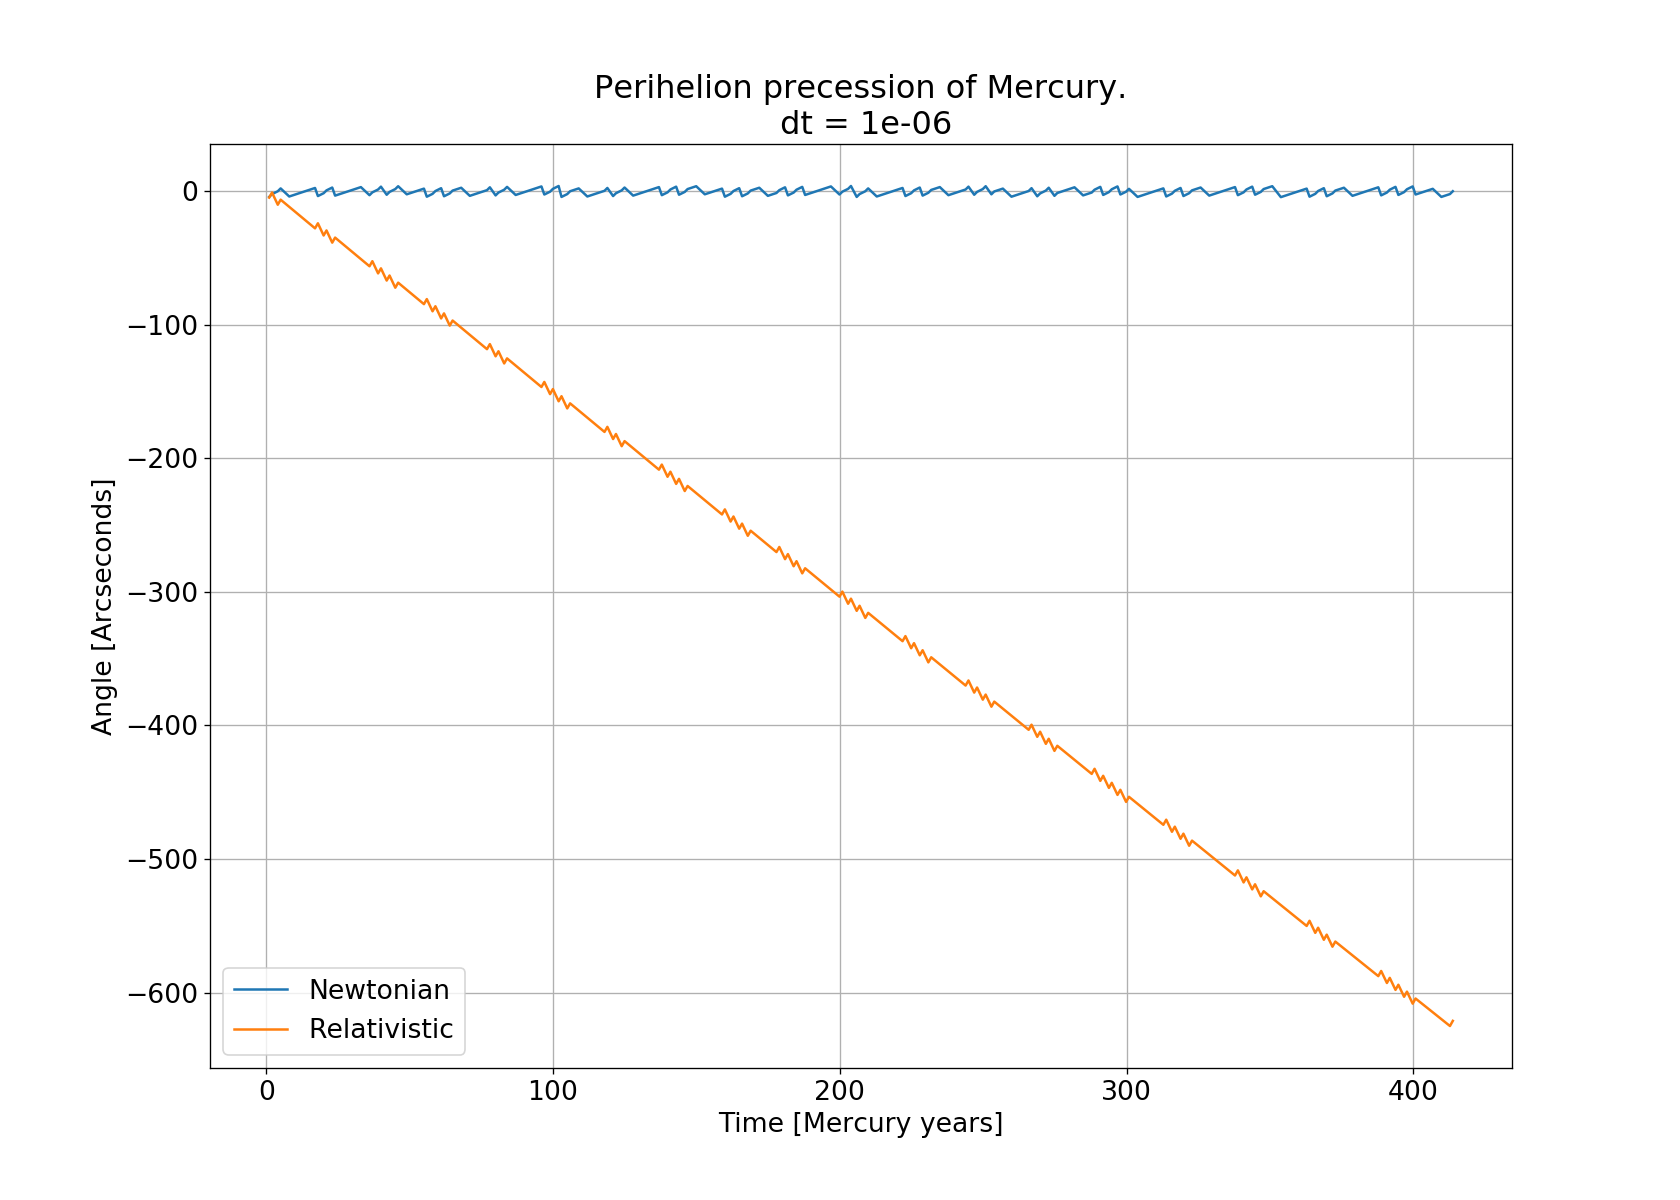
\includegraphics[scale=0.4]{mercury_perihelion_comparison_dt_1e_06_f.png}
\caption{Plot of the perihelion precession of Mercury for the Newtonian and the relativistic force with a time step of 0.000001. The angular velocity is approximately 43 arcseconds/century with the relativistic correction. This fits beautifully to observations.  \label{fig:mercury}}
\end{figure}

\section{Conclusion}
The first goal of the project was to determine the accuracy of the Forward Euler and Velocity Verlet algorithms. He latter was found to be superior in terms of accuracy, even though the Forward Euler was faster and easier to implement. What makes the Velocity Verlet superior is the fact that it produces stable orbits at step sizes up to $dt = \mathrm{0.01}$, while the Forward Euler needed much finer step sizes to produce close to stable orbits. 

The escape velocity of the Earth was calculated using the Velocity Verlet algorithm to see if it matched the theoretical one. The calculated value was indeed close, proving that the algorithm is accurate in simulating the Solar System. It was also proven accurate when checking for conservation of total energy and angular momentum. The Forward Euler failed to do this. It is important that these quantities are conserved when dealing with gravitational forces. 

For the three-body problem of the Sun-Earth-Jupiter system, it was found that Jupiter indirectly influences Earth's orbit by slightly changing the position of the Sun. This effect was greatly increased when Jupiter's mass was increased ten and thousandfold. 

Lastly, Mercury's precessing orbit was plotted with and without a relativistic correction to the gravitational force. It's angular velocity of 43 arcseconds was confirmed in these calculations, thereby confirming observations and general relativity. 




%-----------------------------------------------------%



\begin{flushleft}

\begin{thebibliography}{}

\singlespacing
\small




  
\bibitem{Bok}
  Morten Hjorth-Jensen,
  Computational Physics,
  August 2015

\bibitem{physics}
  Young, Freedman and Zemansky,
  University Physics with Modern Physics,
  Addison-Wesley,
  2004

\bibitem{Hafr}
  Anders Hafreager (2016),
  Project 3 class example,
  \url{https://github.com/andeplane/solar-system},
  accessed: 16th of October 2017  
  
\bibitem{NASA}
  Jet Propulsions Laboratory,
  Horizons Web Interface,
  \url{https://ssd.jpl.nasa.gov/horizons.cgi},
  accessed: 16th of October 2017
  
\end{thebibliography}
\end{flushleft}



\end{document}




















